\documentclass[11pt,a4paper]{article}
\usepackage[T1]{fontenc}
\usepackage[utf8]{inputenc}
\usepackage[sc]{mathpazo}
\usepackage{amsmath,amssymb,amsthm,mathtools}
\usepackage[margin=26mm,headheight=15pt]{geometry}
\usepackage{microtype,booktabs,longtable,array,enumitem}
\usepackage{graphicx,xcolor,fancyhdr,xurl,needspace}
\usepackage[section]{placeins}
\usepackage[colorlinks=true,linkcolor=blue!45!black,citecolor=blue!45!black,
 urlcolor=blue!45!black,bookmarksnumbered=true]{hyperref}
\definecolor{ink}{RGB}{24,47,68}
\definecolor{accent}{RGB}{16,103,122}
\hypersetup{pdftitle={Noisy Parity on Finite and Infinite Cubes},
 pdfauthor={OpenAI ChatGPT; prepared for Vladimir Reshetnikov},
 pdfsubject={Exact coloring, inspection budgets, asymptotics, and measurable choice}}
\newtheorem{theorem}{Theorem}[section]
\newtheorem{lemma}[theorem]{Lemma}
\newtheorem{proposition}[theorem]{Proposition}
\newtheorem{corollary}[theorem]{Corollary}
\theoremstyle{definition}
\newtheorem{definition}[theorem]{Definition}
\newtheorem{example}[theorem]{Example}
\newtheorem{question}[theorem]{Research question}
\theoremstyle{remark}
\newtheorem{remark}[theorem]{Remark}
\newcommand{\N}{\mathbb N}
\newcommand{\R}{\mathbb R}
\newcommand{\E}{\mathbb E}
\newcommand{\Pbb}{\mathbb P}
\newcommand{\Ftwo}{\mathbb F_2}
\newcommand{\Fin}{\operatorname{Fin}}
\newcommand{\cX}{\mathcal X}
\newcommand{\Win}{\operatorname{Win}}
\newcommand{\Inf}{\operatorname{Inf}}
\newcommand{\Var}{\operatorname{Var}}
\newcommand{\supp}{\operatorname{supp}}
\newcommand{\dist}{\operatorname{dist}}
\newcommand{\one}{\mathbf 1}
\newcommand{\pin}{b71545625fedc631edc2ead542abbfba72eb6063}
% Added by the ProveIt write phase (batch 114, 5 October 2026): dated notes
% marked [write], and a command for repository paths and commits.
\newcommand{\file}[1]{\nolinkurl{#1}}
\newenvironment{writenote}[1][]{\par\smallskip\begingroup\small
 \noindent\textbf{[write]}\if\relax\detokenize{#1}\relax\else~\textbf{#1.}\fi\ }%
 {\par\endgroup\smallskip}
\setlist{itemsep=3pt,topsep=5pt}
\setlength{\parskip}{4pt}
\setlength{\parindent}{1.2em}
\renewcommand{\arraystretch}{1.15}
\newcolumntype{L}[1]{>{\raggedright\arraybackslash}p{#1}}
\allowdisplaybreaks[2]
\pagestyle{fancy}
\fancyhf{}
\fancyhead[L]{\small\textsc{Noisy parity}}
\fancyhead[R]{\small Finite and infinite cubes}
\fancyfoot[C]{\small\thepage}
\begin{document}
\hypersetup{pageanchor=false}
\begin{titlepage}
\centering
\vspace*{12mm}
{\color{accent}\large MATHEMATICAL RESEARCH REPORT\par}
\vspace{13mm}
{\color{ink}\Huge\bfseries Noisy Parity on Finite\\[4pt] and Infinite Cubes\par}
\vspace{8mm}
{\Large Exact coloring, inspection budgets,\\[3pt]
 asymptotic laws, and measurable choice\par}
\vspace{15mm}
{\large Prepared for Vladimir Reshetnikov\par}
\vspace{3mm}
{AI-assisted mathematical development and exposition\par}
\vspace{3mm}
{5 October 2026\par}
\vspace{13mm}
\begin{minipage}{0.91\textwidth}
\small
\textbf{Abstract.}
A configuration consists of finitely or countably many independent fair bits.
One bit is deliberately flipped, with a prescribed distribution over its
location, and independent noise is then applied to every coordinate.
We ask for a single binary labeling that changes its value as often as
possible. For homogeneous noise we solve the optimization exactly, classify
the optimizing degrees, and determine the exact success attainable with
any average inspection budget. A general spectral simulation explains why
adaptive inspection cannot improve that budget frontier: a distribution over
finite parity functions reproduces every XOR-noise response of a measurable
Boolean rule, at no larger expected inspection cost.

The infinite form exhibits two different boundaries. Without noise,
measurable success has supremum one but no maximizer, while an infinite
parity function gives pointwise perfection under a suitable choice principle.
Homogeneous positive noise produces finite measurable optimizers.
Summable coordinate-dependent noise has a different exact classification:
optimization over all coordinate subsets compactifies optimization over finite
subsets, and measurable attainment can fail even though a nonmeasurable rule
has a measurable, optimal success event. We also derive finite-size
transitions, logarithmically periodic corrections for geometric challenge
weights, and power-law and lattice corrections for Zipf weights.

All principal results for the stated models are proved. The parity and Fourier
foundations are classical and explicitly credited. The contribution is a
designed problem, its complete solution in the stated models, and derived
extensions; historical priority is not established. The report is unrefereed
and is not a Lean or Rocq formalization.
\end{minipage}
\vfill
{\small Repository reference: ProveIt, snapshot \texttt{b71545625}\par}
\end{titlepage}
\hypersetup{pageanchor=true}
\begin{writenote}[Status and trust boundary, added 5 October 2026, batch~114]
This manuscript is filed in ProveIt as the single-source research report
\file{noisy-parity-cubes} of the research-report collection (provenance,
the repository claims checked against the current tree, the two lemmas that
the report \file{measurable-box-games} already proves, reading conventions
and the collected non-claims are in Section~\ref{np:sec:provenance}). It is
AI-assisted (the title page says ``AI-assisted mathematical development and
exposition''; the PDF author field reads ``OpenAI ChatGPT; prepared for
Vladimir Reshetnikov''), unrefereed and \emph{not formalized}: no Lean or
Rocq declaration states any theorem of this report. \emph{What rests on
what.} Every theorem has a written proof; the Fourier and influence
machinery is classical~\cite{odonnell}, and the parity-function and
measurable-colouring facts of Section~\ref{np:found:section} are classical
and credited~\cite{glr,serafin,conleymiller}. The exhaustive finite checks
(dimensions $1$--$4$) and the 65-digit asymptotic diagnostics of
Section~\ref{np:sec:checks} support the finite formulas and the signs and
sizes of the asymptotic coefficients; no infinite statement rests on a
computation. The write adds two remarks with proofs:
Remark~\ref{np:rem:deterministic} (under strictly decreasing weights no
deterministic tree attains the inspection frontier at a non-integer budget
below $K$) and Remark~\ref{np:rem:gap-shrinks} (the stability gap of
Theorem~\ref{np:thm:stability} tends to zero as $\eta\downarrow0$ on a
countable cube); it also adds the second-route notes at
Lemma~\ref{np:lem:query} and after Corollary~\ref{np:cor:simulation}, and
Section~\ref{np:sec:further}, which states every open item as a question.
Nothing in the source was found to be wrong.
\end{writenote}
\begingroup\small\setlength{\parskip}{0pt}\tableofcontents\endgroup
\clearpage

\section{The problem and its mathematical setting}\label{np:sec:intro}

\subsection{A puzzle with a finite and an infinite life}

Imagine a panel of lamps. A rule assigns every possible lamp configuration
one of two labels. The same rule is used whenever the panel is inspected.
A referee chooses a random fair configuration, deliberately toggles one
lamp, and then applies random faults. The goal is for the two configurations
to receive opposite labels.

For a finite panel without faults, the parity of the number of lit lamps
solves the problem perfectly. Adding faults changes the optimization:
using more lamps makes it more likely that the deliberate toggle is
noticed, but also makes the parity vulnerable to more accidental toggles.
An infinite panel raises a second issue. Parity of infinitely many lit
lamps is not an ordinary convergent sum. There are choice-based parity
labelings, but they have strong failures of measurability.

This report asks three precise questions.
\begin{enumerate}
\item What is the largest probability that the label changes, for a given
distribution of the deliberate toggle and a given noise rate?
\item What can be achieved when the expected number of inspected lamps is
bounded, even if the choice of the next lamp depends on earlier observations?
\item Which aspects survive on a countably infinite panel, and where do
measurability and choice change attainment of the optimum?
\end{enumerate}
The finite game is a weighted maximum-cut problem on a binary cube. Its
infinite form connects this elementary puzzle with Fourier analysis,
decision trees, asymptotic optimization, and descriptive set theory.

\subsection{Why this is a plausible Glazer--ProveIt intersection}

Glazer's public author biography explicitly identifies choice paradoxes,
formal systems, proof-assistant foundations, and puzzles in finite and
infinite settings as interests \cite{glazerbio}. His box-game paper supplies
a direct mathematical connection between prediction and choice
\cite{glazerbox}. These are reasons to expect interest in the present
problem, rather than an assertion of his endorsement or involvement.

Two inspected parts of ProveIt provide concrete points of contact.
The module \path{ThueMorseBooleanCube.lean} proves finite binary-cube
product identities, including the signed Thue--Morse product and a
binary-weight enumerator \cite{repocube}. Under binary enumeration,
the parity character used here is exactly the finite Thue--Morse sign.
The repository's research report \emph{Countable Information,
Uncountably Many Boxes} studies measurable prediction, finite decision
trees, and inspection budgets \cite{repobox}. Its README describes the
report as unrefereed and unformalized. We use this as context, not as an
assumed theorem dependency.

\begin{writenote}[Checked against the current tree, 5 October 2026]
Both statements are correct at the pin and still at the current tree: the
two cited files are byte-identical at the pin and at the write. The cited
Lean module proves the three finite product identities named in
Section~\ref{np:sec:formalization}, and the sign it uses is
$(-1)^{\text{binary weight of }n}$, so the parity character of the first
$m$ coordinates is that sign under binary enumeration of $\{0,1\}^m$.
A neighbouring module, not cited by the source, proves Walsh-character
orthogonality on the same dyadic block. The report
\file{measurable-box-games} has five Parts (at the pin as now), and its
Part~IV proves the
two classical lemmas that this report re-proves in
Section~\ref{np:sec:spectral}. Details, with declaration names, are in
Section~\ref{np:sec:provenance}.
\end{writenote}

The principal results below concern a single labeling evaluated at two
correlated configurations. They do not re-prove the repository's
infinite-hat surplus or box-guessing budget theorems. All proofs needed for
our game are given here.

\subsection{What is classical and what is established here}

Walsh expansion, spectral samples, noise operators, and influence identities
are standard \cite{odonnell}. Infinite parity functions and their
choice-sensitive behavior are also established literature
\cite{glr,serafin}; the measurable chromatic obstruction is classical
\cite{conleymiller}.

The report formulates a weighted noisy-parity puzzle and proves the exact
optimization, inspection frontier, optimizer structure, noise asymptotics,
and summable-noise attainment results stated below. These are mathematical
claims in the specified models, not claims that a named published open
problem has been settled. A targeted search found the relevant classical
machinery but did not establish historical priority for the precise
formulation and assembled results.

\subsection{Provenance, repository context and reading conventions}
\label{np:sec:provenance}
\begin{writenote}[Added 5 October 2026, batch~114]
\emph{Provenance.} This report is built from one manuscript, the archive
\file{Noisy_Parity_Finite_and_Infinite_Cubes.zip} (474{,}728 bytes, SHA-256 beginning
\file{c58216c1}; wrapper directory \file{noisy_parity/}, 13
files, 639{,}515 bytes unpacked), which arrived in ProveIt's
\file{docs/incoming} drop zone in commit \file{2399df2bd} (``New research
reports'', 5~October 2026). It is not part of a numbered report bundle. The
intake placed it as batch~114 in commit \file{99053b5d1}. The text is the
delivered \file{noisy_parity.tex} (2{,}298 lines, 97 labels, all already
prefixed \file{np:}), shipped as \file{article.tex}; the three figure PDFs,
the three programs and their three recorded outputs are shipped
byte-identical (\file{build.sh} in \file{code/}). The delivered 32-page
\file{noisy_parity.pdf} is not shipped and is retrievable from the arrival
commit; the package has no checksum manifest. The package is ``Prepared for
Vladimir Reshetnikov'' (authorship, kept here, not an author line) and
pins ProveIt commit \texttt{\pin} (title page, Appendix~\ref{np:app:package},
bibliography), an ancestor of the current tree. Single source, so no merge
choice was made.

\emph{The repository claims, checked at the current tree.}
(i)~\file{Analysis/FabiusFunction/Lean/FabiusFunction/ThueMorseBooleanCube.lean}
(97 lines, namespace \file{Fabius}; blob \file{3527bee8} at the pin and
now) proves four theorems: \file{prod_one_add_eq_sum_powerset}
($\prod_{j\in S}(1+x_j)=\sum_{T\subseteq S}\prod_{j\in T}x_j$),
\file{prod_one_add_mul_pow}
($\prod_{j<m}(1+uz^{2^j})=\sum_{n<2^m}u^{w(n)}z^n$ over every commutative
semiring, $w$ the binary weight),
\file{prod_one_sub_pow_eq_sum_thueMorseSign}
($\prod_{j<m}(1-z^{2^j})=\sum_{n<2^m}\varepsilon(n)z^n$ over every
commutative ring) and \file{sum_pow_binaryWeight_eq_one_add_pow}
($\sum_{n<2^m}u^{w(n)}=(1+u)^m$); the sign is
$\varepsilon(n)=(-1)^{w(n)}$, the definition of \file{thueMorseSign} in
\file{FabiusFunction/Arithmetic.lean}. The source's description is
correct, and so is its reading that $\chi_{[m]}$ is $\varepsilon$ under
binary enumeration of $\{0,1\}^m$. \emph{Observation of the write, not used
by the source:} over $\mathbb Q$ or $\R$, the last identity with
$u=-\eta/(1-\eta)$, multiplied by $(1-\eta)^k$, is
$\sum_{n<2^k}\eta^{w(n)}(1-\eta)^{k-w(n)}(-1)^{w(n)}=(1-2\eta)^k$, that is
$\E\chi_S(B)=a^{|S|}$ for $|S|=k$, the noise factor
of~\eqref{np:eq:eigenvalue}. (ii)~The neighbouring module
\file{ThueMorseWalsh.lean} (353 lines, blob \file{63a333d6} at the pin and
now; not cited by the source) proves
\file{sum_neg_one_pow_binaryWeight_land}: for $a<2^m$,
$\sum_{n<2^m}(-1)^{w(a\,\&\,n)}$ is $2^m$ if $a=0$ and $0$ otherwise (the
vanishing of a nontrivial character sum, in binary encoding; the
orthogonality $\E\chi_S\chi_T=\one_{\{S=T\}}$ follows from it by
$\chi_S\chi_T=\chi_{S\triangle T}$, which that file does not state), the
masked character sum \file{sum_pow_binaryWeight_mul_pow_binaryWeight_land}
and the one-point Walsh spectrum \file{sum_thueMorseSign_mul_walsh} of the
full parity. (iii)~No Lean or Rocq file of the repository proves Walsh
inversion or Parseval for arbitrary functions on a binary cube, or treats
influences, decision trees or noise channels (searches for
\emph{walsh}, \emph{parseval}, \emph{plancherel}, \emph{influence},
\emph{decision tree}, \emph{noise} in \file{*.lean} and \file{*.v}; the
Walsh-basis lemma of \file{Combinatorics/Ramsey/Lean/GowersSzemeredi/}
concerns Gowers' Lemma~15.1 over $\mathbb Z/N$ and is unrelated). So the
statement of Section~\ref{np:sec:formalization} that its modules are
proposed, not present, is still true; (i) and (ii) supply ingredients of its
first layer only. This report shares no declaration with any formal file
and none of its statements is formalized. (iv)~The report
\file{SetTheory/Cardinals/docs/reports/ordinals-and-order-types/measurable-box-games}
(README blob \file{04ce7e69} at the pin and now) does study measurable
prediction, finite decision trees and inspection budgets (its Parts~I, IV
and~V), and its README calls it ``AI-assisted, unrefereed, not
formalized''.

\emph{Second routes.} Two standard lemmas proved here are already proved
in Part~IV of \file{measurable-box-games}~\cite{repoboxart}, where they are
credited as classical: Lemma~\ref{np:lem:query} (influence at most the
expected number of inspections, with its per-coordinate form used in
Proposition~\ref{np:prop:equality}) is the second display of its
Lemma~64.1, \file{mbg:insp:var-covariance} (source~04 of that Part); the
statement after Corollary~\ref{np:cor:simulation} that a depth-$d$ tree
has Walsh degree at most $d$ is its Lemma~49.1, \file{mbg:qry:lem:degree}
(source~06). The proofs here are independent one-paragraph arguments of the
same kind and are kept as second routes; notes at both places point there.
That report works with $\pm1$ hats and $\chi_A=\prod_{j\in A}x_j$, this one
with bits and $\chi_S=(-1)^{\sum_{i\in S}x_i}$; its $\Inf_j(g)=
\E(\partial_jg)^2$ equals the flip influence $\Inf_j$ used here for
$\pm1$-valued $g$. It uses the Walsh expansion and a noise operator for
degree and hypercontractive estimates; the write found there no counterpart
of the spectral simulation (Theorem~\ref{np:thm:fourier},
Corollary~\ref{np:cor:simulation}) or of the other results of this report.

\emph{See also.} \file{ordinals-and-order-types/robust-neutral-choice}
(batch~114, placed in the same commit, independent source) meets this report
only in side sections: choice-built labels invariant under finite changes on
$2^{\N}$, their failure of measurability and the Baire property, and a
biased-product threshold there
($\sum_i(p_i-\tfrac12)^2=\infty$ for its neutral $E_0$-invariant rules)
beside Proposition~\ref{np:found:biased} here
($\sum_i\min(q_i,1-q_i)<\infty$ for total parity labels). These concern
different symmetries; neither is an instance of the other. Neither source
cites the other.

\emph{What the write changed.} It added the notes marked [write], this
subsection, Remarks~\ref{np:rem:deterministic} and~\ref{np:rem:gap-shrinks}
(each the last numbered statement of its section),
Section~\ref{np:sec:further} with questions Q13--Q15, labels on the source's
Q1--Q12 (with a \texttt{ref} key on their list, which does not
change the output), two preamble definitions and two bibliography entries.
No statement, proof or number of the source was changed.

\emph{The external sources, as the write read them} (5~October 2026).
Geschke, Lubarsky and Rahn~\cite{glr} (manuscript dated March~13, 2015):
Lemma~5 proves that a strategy with at most one mistake exists if and only
if a parity function exists, Corollary~9(b) that a parity function exists if
and only if there is a transversal of $E_{\mathrm{ev}}$-classes within
$E_0$-classes (the equivalence of
Proposition~\ref{np:found:choice}), and Question~12 asks whether ZF plus a
parity function gives a free ultrafilter or an $E_0$-transversal.
Serafin~\cite{serafin} (arXiv v2, 2~December 2023): Theorem~1, ``Assuming
the consistency of the existence of an inaccessible cardinal'', gives a
model with a parity function and neither a nonprincipal ultrafilter on $\N$
nor an $E_0$-transversal (``otherwise known as a Vitali set''); his
Section~2 makes ``model of set theory'' mean a model of ZF+DC; he presents
the theorem as the answer to that question. So the two literature
statements of Section~\ref{np:found:section} are accurate as cited. Not read
by the write: Conley--Miller~\cite{conleymiller}, O'Donnell~\cite{odonnell},
OSSS~\cite{osss}, DLMF~25.11~\cite{dlmf} and the Epoch AI
biography~\cite{glazerbio}.
\end{writenote}

\begin{writenote}[Reading conventions, 5 October 2026]
The source reuses several letters; each meaning is fixed by its section.
No symbol was renamed. ``Success'' always means \emph{disagreement},
$f(X)\ne f(Y)$; $\Win$ is not the probability of a correct label.
\end{writenote}
{\small
\begin{longtable}{@{}L{.13\textwidth}L{.50\textwidth}L{.28\textwidth}@{}}
\toprule
Symbol & Meanings (where) & Do not read as\\
\midrule
\endhead
$a$, $a_i$, $a(S)$ & $a=1-2\eta$ (homogeneous noise); $a_i=1-2\eta_i$ and
 $a(S)=\prod_{i\in S}a_i$ (summable noise, Section~\ref{np:found:section}) &
 \\
$A$, $B$ & $A=a(\N)$ (Theorem~\ref{np:found:full-parity}); Fourier
 coefficients $A,B$ (proofs of Theorems~\ref{np:thm:optimizers},
 \ref{np:thm:stability}); an independent set (proof of
 Proposition~\ref{np:found:regularity}); the event
 $A_n=\{\supp D\subseteq[n]\}$ (Theorem~\ref{np:thm:finiteperturb}) &
 \\
$b_k$, $b$ & $b_k=2P_k-1$; the modal sequence $b$ (proof of
 Proposition~\ref{np:found:biased}); $b_0(\rho)$ (Zipf proof) &
 \\
$B$ & the noise vector $(B_i)$; the event $B_n$ (proof of
 Theorem~\ref{np:found:summable-theorem}); the Bernoulli polynomial $B_2$
 (Theorem~\ref{np:asym:lattice-theorem}) &
 \\
$C$ & Zipf constant; $C(f)$, $C_n(f)$ minimum expected tree cost; a
 cylinder; an $E_0$-class with representative $r_C$ & \\
$D$, $d$ & a random finite-support flip vector
 (Section~\ref{np:sec:finiteperturb}); $D=\alpha/s+2\varepsilon$ (Zipf);
 the coefficient $D$ of Q8; $d_k=2ap_{k+1}-(1-a)b_k$; the rounding offset
 $d$ in $k=Rs+d$ & \\
$\varepsilon$, $\epsilon$ & the score deficit of
 Theorem~\ref{np:thm:stability}; the Zipf scale $\varepsilon=\eta R$; the
 zero-noise deficit $\epsilon(f)$ & three unrelated quantities\\
$\alpha$ & the tail index; the spectral mixture $\alpha(S)$; the
 probabilities $\alpha_n$ of $B_n$ or $A_n$ & \\
$F_k$, $F(S)$ & $F_k=a^kb_k$; $F(S)=(2p(S)-1)a(S)$; with equal noise
 rates $F_k=F([k])$ & $F_k>0$ (false at $k=0$)\\
$G$ & the frontier $G(c)$; $G_0(\rho)$ (Zipf proof) & \\
$h$ & $h_k=p_k/b_k$; a total parity function $h$
 (Corollary~\ref{np:cor:uniformchoice}); sections $h_{j,z}$ & \\
$K$, $k_\eta$ & $K=K_\eta$ the \emph{smallest} maximizing degree;
 $k_\eta$ any chosen maximizing degree (Section~\ref{np:asym:section}) &
 the unique maximizer (an adjacent tie can occur)\\
$L$, $\mathcal L$ & $L(\eta)=1-V(\eta)$; label classes $\mathcal L_\mu
 \subseteq\mathcal L_{\mathrm{evt}}$; smooth losses $\mathcal L_0$,
 $\mathcal L(x)$ & a measurable success event as a measurable label\\
$M$, $\mathcal M$ & $\mathcal M$ the optimal family of finite sets
 (Section~\ref{np:sec:stability}); $M=\max_SF(S)$; a truncation size $M$
 (Section~\ref{np:sec:spectral}); $M_0$ (Zipf) & \\
$q$ & biased coordinate probabilities $q_i$
 (Proposition~\ref{np:found:biased}); $q(S)$
 (Theorem~\ref{np:thm:finiteperturb}) & \\
$R$ & the shared seed; $R=(C/\eta)^{1/\alpha}$; $R_n=\sum_{i>n}\eta_i$ & \\
$s$ & $s(c)$ (Theorem~\ref{np:asym:uniform-limit}); the saddle root
 $s_\alpha(\varepsilon)$ & \\
$T$, $t_k$ & the operator $T_\rho$; the Zipf tail $T(x)$; $t_k=1-P_k$ & \\
$u$ & $u_\rho(S)$; $u_\eta=\{x_\eta\}$; the lattice phase $\{Rs\}$; the
 argument of $g_\alpha$; a finite-support translation & \\
$V$ & optimal scores of different models: $V(p,\eta)$, $V_\rho(c)$, $V_n$,
 $V_\infty$, $V(\eta)$, $V_n(\eta)$, and $V$ in
 Theorem~\ref{np:found:summable-theorem} & one quantity\\
$\eta$ & the noise rate (here); in
 \file{robust-neutral-choice} $\eta$ is an unrelated tolerance & \\
$\Inf_i$ & flip influence, a probability & a variance of a
 non-Boolean function\\
\bottomrule
\end{longtable}}

\begin{writenote}[What is not claimed, collected from the source]
The Fourier, spectral-sample and influence machinery is classical and
credited to O'Donnell; infinite parity functions and their choice behaviour
are classical (Geschke--Lubarsky--Rahn, Serafin), and the measurable
chromatic obstruction is classical (Conley--Miller). The puzzle is designed;
historical priority is not established; it is not a named open problem,
not refereed, not a Lean or Rocq formalization, and claims no endorsement or
involvement of Elliot Glazer. The spectral simulation neither computes $f$
nor preserves correlations of three or more inputs, and computing the
spectral distribution is a separate problem. The expected-budget optimum is
not identified with the optimum over deterministic trees under an average
cost constraint. The restricted parity-choice principle is not equated with
AC or with choice for arbitrary pairs; ultrafilter or
$E_0$-transversal constructions are sufficient, not necessary; no new choice
equivalence is inferred. The stability gap may shrink as $\eta\to0$ (the
write proves it does, Remark~\ref{np:rem:gap-shrinks}). There is no
countably infinite uniform model. The Zipf formula is not read as resolving
terms below its remainder. The Decimal checks are not interval
certificates, and the plots illustrate proved formulas without being
evidence for them. The formalization table proposes modules. The requested
LinkedIn page gave no usable content; Glazer's interests are taken from his
Epoch AI biography. No repository modification or communication with a
named mathematician was part of the deliverable.
\end{writenote}

\section{Rules, notation, and the main answers}\label{np:sec:rules}

Let \(I=[n]=\{1,\ldots,n\}\), or \(I=\N=\{1,2,\ldots\}\), and let
\[
 \cX=\{0,1\}^{I},\qquad
 \mu=\bigotimes_{i\in I}\operatorname{Bernoulli}(1/2).
\]
We allow the completion of this probability measure. Addition
\(\oplus\) means coordinatewise addition modulo two. Write \(e_i\) for
the configuration supported at the single coordinate \(i\).

Fix positive probabilities \(p_i\) with \(\sum_i p_i=1\), ordered so that
\(p_1\ge p_2\ge\cdots\). In the infinite case such an ordering exists:
there are only finitely many probabilities above any positive threshold.
There is no appeal to a uniform probability distribution on \(\N\).
Define
\[
 P_k=\sum_{i=1}^k p_i,\quad P_0=0,\quad
 t_k=1-P_k,\quad b_k=2P_k-1.
\]

\begin{definition}[The homogeneous noisy-parity experiment]
Draw \(X\sim\mu\), an index \(J\) with \(\Pbb(J=i)=p_i\), and
independent bits \(B_i\sim\operatorname{Bernoulli}(\eta)\), all independently.
Set
\[
 Y=X\oplus e_J\oplus B.
\]
For a measurable labeling \(f:\cX\to\{-1,1\}\), its score is
\[
 \Win_{p,\eta}(f)=\Pbb\bigl(f(X)\ne f(Y)\bigr).
\]
The same labeling is used at both inputs. A random labeling uses one
shared seed \(R\), independent of \(X,J,B\), and applies \(f_R\) twice.
\end{definition}

Both \(X\) and \(Y\) have law \(\mu\). When \(I=\N\) and \(\eta>0\),
infinitely many noise bits are one almost surely. The definition is still
ordinary product probability: each coordinate of \(Y\) is a measurable
function of the sampled variables.

The same-rule condition matters. Allowing two unrelated labelings would
permit opposite constants and give a score of one without any inspection.
Sharing the seed likewise specifies the resource model: separate fresh
output coins would be a different game.

Put \(a=1-2\eta\). For \(0\le\eta<1/2\), define
\begin{equation}\label{np:eq:wk}
 F_k=a^k b_k,\qquad w_k=\frac{1+F_k}{2},
 \qquad F_0=-1,\quad w_0=0.
\end{equation}
The parity on the \(k\) heaviest coordinates is
\[
 \chi_{[k]}(x)=(-1)^{x_1+\cdots+x_k}.
\]

\Needspace{9\baselineskip}
\begin{theorem}[Exact value and exact inspection frontier]\label{np:thm:main}
For \(0<\eta<1/2\), let \(K\) be the smallest index maximizing \(w_k\),
with \(0\le k\le n\) in the finite case. Then:
\begin{enumerate}
\item The optimal measurable score is \(V(p,\eta)=w_K\), and
\(\chi_{[K]}\) attains it.
\item The maximizing degrees are either \(K\) alone, or \(K,K+1\).
The index \(K\) is finite even when \(I=\N\).
\item Let \(G(c)\) be linear between successive points
\((k,w_k)\), \(0\le k\le K\), and constant with value \(w_K\) for \(c\ge K\).
Among all exact adaptive shared-randomized labeling procedures with expected
inspection cost at most \(c\) per evaluation, the optimal score is \(G(c)\).
\end{enumerate}
\end{theorem}

Here an exact procedure reads individual coordinates, may adapt its next
query to the answers already seen, and terminates with its chosen label
almost surely. Cost counts distinct coordinate inspections; repeated
queries can be cached. Preprocessing and random-seed generation are free.
For noninteger \(c<K\), the optimum is attained by choosing the parities
of sizes \(\lfloor c\rfloor\) and \(\lceil c\rceil\) with the corresponding
linear interpolation probabilities.

The proof occupies Sections~\ref{np:sec:spectral}--\ref{np:sec:budget}.
The infinity and noise boundaries are as follows.

\begin{center}
\small
\begin{tabular}{@{}L{.24\textwidth}L{.30\textwidth}L{.36\textwidth}@{}}
\toprule
Setting & Measurable labelings & Additional conclusion\\
\midrule
Finite, \(\eta=0\)& Perfect parity exists & Inspect every challenged coordinate.\\
Countably infinite, \(\eta=0\)& Supremum \(1\), not attained
 & Choice-based parity is pointwise perfect.\\
Countably infinite, \(0<\eta<1/2\)& A finite optimum is attained
 & Every measurable optimizer has finite dependence, up to a null set.\\
Summable coordinate noise& Compact optimization over all subsets
 & The supremum can require an infinite, nonmeasurable labeling to be attained.\\
\bottomrule
\end{tabular}
\end{center}

\section{A general spectral simulation}\label{np:sec:spectral}

\subsection{The countable Fourier basis}

For a finite subset \(S\subseteq I\), define
\[
 \chi_S(x)=(-1)^{\sum_{i\in S}x_i}.
\]
The empty character is identically one. Independence gives
\(\E_\mu[\chi_S\chi_T]=\one_{\{S=T\}}\). In finite dimension these
characters form a basis by counting dimensions.

In countable dimension, functions of the first \(m\) bits are spanned by
\(\chi_S\), \(S\subseteq[m]\). Conditional expectations onto these
coordinate sigma-algebras converge in \(L^2\), so their union is dense.
Consequently every real \(f\in L^2(\mu)\) has the expansion
\[
 f=\sum_{S\in\Fin(I)}\widehat f(S)\chi_S,\qquad
 \widehat f(S)=\E_\mu[f\chi_S],\qquad
 \sum_S\widehat f(S)^2=\|f\|_2^2.
\]
For a Boolean \(f\), the final sum is one. The family of finite subsets is
countable, so its squared coefficients are an ordinary discrete
probability distribution.

\begin{theorem}[Every XOR-noise response is a parity mixture]
\label{np:thm:fourier}
Let \(Z\) have any probability law \(\rho\) on \(\cX\), independently of
\(X\sim\mu\), and put \(Y=X\oplus Z\). For every measurable Boolean \(f\),
\begin{equation}\label{np:eq:spectral}
 \Win_\rho(f)=
 \sum_{S\in\Fin(I)}\widehat f(S)^2
 \frac{1-\E_\rho\chi_S(Z)}2.
\end{equation}
Thus a shared random parity \(\chi_S\), with
\(\Pbb(S=T)=\widehat f(T)^2\), reproduces the score of \(f\) for every
law \(\rho\) simultaneously.
\end{theorem}

\begin{proof}
The convolution operator
\(T_\rho g(x)=\E_\rho[g(x\oplus Z)]\) is an \(L^2\) contraction.
Indeed Jensen's inequality followed by invariance of \(\mu\) gives
\[
 \|T_\rho g\|_2^2
 \le \E_{\mu,\rho}|g(X\oplus Z)|^2=\|g\|_2^2.
\]
Every character is an eigenfunction:
\[
 T_\rho\chi_S=(\E_\rho\chi_S(Z))\chi_S.
\]
Apply this to finite Fourier sums and pass to \(L^2\) limits to get
\[
 \E[f(X)f(Y)]
 =\langle f,T_\rho f\rangle
 =\sum_S\widehat f(S)^2\E_\rho\chi_S(Z).
\]
The series is absolutely convergent because
\(|\E_\rho\chi_S(Z)|\le1\). Finally,
\(\one_{\{u\ne v\}}=(1-uv)/2\) for \(u,v\in\{-1,1\}\), proving
\eqref{np:eq:spectral}. The distribution of \(S\) depends only on \(f\);
therefore the same simulation works for every noise law.
\end{proof}

The theorem matches a two-input response profile. It does not assert that
the simulated parity computes the original labeling, nor that it preserves
arbitrary three-input or higher correlations. Computing the spectral
distribution efficiently is a separate algorithmic question. The
squared-coefficient distribution is the classical spectral sample
\cite{odonnell}; the operational statement here is its application to this
labeling game.

\subsection{Why the simulation never uses more expected inspections}

Define the flip influence of coordinate \(i\) by
\[
 \Inf_i(f)=\Pbb_\mu\bigl(f(X)\ne f(X\oplus e_i)\bigr),\qquad
 \mathcal I(f)=\sum_i\Inf_i(f).
\]
Fourier expansion of \(f(x)-f(x\oplus e_i)\) gives
\[
 \Inf_i(f)=\sum_{S\ni i}\widehat f(S)^2.
\]
Tonelli's theorem therefore gives the possibly infinite identity
\begin{equation}\label{np:eq:influence}
 \mathcal I(f)=\sum_S |S|\widehat f(S)^2.
\end{equation}

\begin{lemma}[Pivotality is paid for by inspection]\label{np:lem:query}
If an exact adaptive procedure computes \(f\) with query count \(Q(X)\),
then \(\mathcal I(f)\le\E Q(X)\).
\end{lemma}
\begin{proof}
If a computation on \(x\) never inspects coordinate \(i\), the same path
and output occur on \(x\oplus e_i\). Thus, except on the null sets where
one of the computations is not exact and terminating,
\[
 \{f(x)\ne f(x\oplus e_i)\}\subseteq
 \{\text{the computation on }x\text{ inspects }i\}.
\]
Finite flips preserve \(\mu\), so these exceptions remain null. Integrating
and summing over \(i\) proves the inequality.
\end{proof}

\begin{writenote}[Second route, 5 October 2026]
This lemma, and its per-coordinate form (\(\Inf_i(f)\) is at most the
probability that coordinate \(i\) is inspected) used in the proof of
Proposition~\ref{np:prop:equality}, are the second display of
Lemma~64.1 (\file{mbg:insp:var-covariance}) in Part~IV of the report
\file{measurable-box-games}~\cite{repoboxart}, proved there by the same
path argument for almost surely terminating deterministic inspection
algorithms and credited as classical. The proof above is an independent
second route; nothing here depends on that report.
\end{writenote}

\begin{corollary}[No advantage from adaptive inspection]
\label{np:cor:simulation}
For every exact adaptive shared-randomized labeling protocol there is
a randomized nonadaptive parity protocol with no larger expected inspection
cost and the same score for every independent XOR perturbation law.
\end{corollary}
\begin{proof}
For a fixed label \(f\), the spectral simulation reads \(|S|\) coordinates,
whose expectation is \(\mathcal I(f)\) by \eqref{np:eq:influence}.
Apply Lemma~\ref{np:lem:query}. For a random label \(f_R\), average the
spectral distributions over the shared seed:
\[
 \alpha(S)=\E_R\widehat f_R(S)^2.
\]
Joint measurability and Tonelli give \(\sum_S\alpha(S)=1\); the same
calculation proves both the score and cost assertions.
\end{proof}

This uses an elementary influence bound, not the stronger
O'Donnell--Saks--Schramm--Servedio inequality \cite{osss}.
A uniform maximum depth is also preserved: a depth-\(d\) decision tree
has Fourier degree at most \(d\), by induction on the root query.
Its spectral sample therefore has size at most \(d\).

\begin{writenote}[Second route, 5 October 2026]
The degree bound is Lemma~49.1 (\file{mbg:qry:lem:degree}) in Part~IV of
\file{measurable-box-games}~\cite{repoboxart}, proved there by the same
induction on the first query (with \(\pm1\) coordinates); the one-line
argument here is a second route.
\end{writenote}

\begin{proposition}[When the cost inequality is equality]
\label{np:prop:equality}
In finite dimension let \(C(f)\) be the minimum expected number of queries
of an exact decision tree under uniform input. Then
\[
 C(f)=\mathcal I(f)
 \quad\Longleftrightarrow\quad
 f=\pm\chi_S\text{ for some }S.
\]
\end{proposition}
\begin{proof}
A parity has influence and optimal cost both equal to \(|S|\).
Conversely choose a minimum-cost tree. If \(f\) is nonconstant, let \(i\)
be its root coordinate. Equality in the sum of the nonnegative
revealment-minus-influence gaps forces \(\Inf_i(f)=1\), since the root
is always read. On a finite cube this means \(f(x\oplus e_i)=-f(x)\)
for every \(x\), so \(f=\chi_{\{i\}}g\) with \(g\) independent of \(i\).
The two restricted functions are \(g\) and \(-g\), with equal minimum
cost. Optimality of the subtrees gives \(C(f)=1+C(g)\), while
\(\mathcal I(f)=1+\mathcal I(g)\). Induction proves that \(g\), and
therefore \(f\), is a signed parity. Constant labels are the empty case.
\end{proof}

\subsection{The resource optimization for an arbitrary perturbation}

Set \(u_\rho(S)=(1-\E_\rho\chi_S(Z))/2\). Corollary
\ref{np:cor:simulation} gives the exact variational formula
\begin{equation}\label{np:eq:generalbudget}
 V_\rho(c)=\sup\left\{
 \sum_S\alpha(S)u_\rho(S):
 \alpha(S)\ge0,\quad\sum_S\alpha(S)=1,\quad
 \sum_S|S|\alpha(S)\le c\right\}.
\end{equation}
In finite dimension this is a finite linear program. An extreme optimal
distribution has at most two nonzero masses: if the cost constraint is
active, three positive masses have a nontrivial perturbation preserving
both total mass and mean cost; if it is inactive, a single mass suffices.

The countable formula is a supremum. Finite mixtures approximate it:
replace all sets of size greater than \(M\) by the empty set, losing score
at most \(c/(M+1)\); then approximate the remaining countable distribution
by finite support. No universal attainment assertion is needed.
For homogeneous noise, the next two sections give an explicit attained
solution.

\section{Solving the homogeneous puzzle}\label{np:sec:exact}

For \(p(S)=\sum_{i\in S}p_i\), independence gives
\begin{equation}\label{np:eq:eigenvalue}
 \E\chi_S(e_J\oplus B)
 =(1-2p(S))\,a^{|S|}.
\end{equation}
The score of a parity is consequently
\[
 \Win_{p,\eta}(\chi_S)=
 \frac{1+a^{|S|}(2p(S)-1)}2.
\]
There is also a direct explanation. The deliberate flip lies in \(S\)
with probability \(p(S)\). The number of accidental flips in \(S\) is
even with probability \((1+a^{|S|})/2\). The two cases give the same formula.

For fixed cardinality \(k\), the score is maximized by selecting the
\(k\) heaviest coordinates, because \(a^k>0\) and
\(p(S)\le P_k\). Theorem~\ref{np:thm:fourier} now proves the upper bound
\(\Win(f)\le\sup_k w_k\), and a maximizing character attains it.
In countable dimension \(P_k\to1\), so some \(F_k\) is positive, while
\(F_k\to0\) when \(0<a<1\). A positive maximum is therefore attained
among finitely many degrees.

\begin{proposition}[Exact cutoff and unimodality]\label{np:prop:cutoff}
For \(0<\eta<1/2\), the sequence \(F_k\) strictly increases to its maximum,
can have one adjacent tie, and then strictly decreases. In finite dimension
set \(p_{n+1}=0\). The first maximizing index is
\begin{equation}\label{np:eq:cutoff}
 K=\min\{k:2a p_{k+1}\le(1-a)(2P_k-1)\}.
\end{equation}
For an index with \(b_k>0\), the equivalent condition for being a
maximizing degree is
\begin{equation}\label{np:eq:threshold}
 \frac{p_{k+1}}{b_{k+1}}\le\eta\le\frac{p_k}{b_k},
\end{equation}
where the left bound is zero at \(k=n\).
\end{proposition}
\begin{proof}
Write
\[
 d_k=2a p_{k+1}-(1-a)b_k.
\]
Then \(F_{k+1}-F_k=a^kd_k\), and
\[
 d_{k+1}-d_k
 =2a(p_{k+2}-p_{k+1})-2(1-a)p_{k+1}<0
\]
where both steps exist. Initially \(d_0>0\); in the infinite case its
limit is \(-(1-a)<0\), and in finite dimension \(d_n=-(1-a)<0\).
This proves the asserted shape and \eqref{np:eq:cutoff}.
Alternatively,
\[
 F_k-F_{k-1}=2a^{k-1}(p_k-\eta b_k).
\]
The ratios \(p_k/b_k\) are strictly decreasing once \(b_k>0\), yielding
\eqref{np:eq:threshold}. A maximizing \(F_k\) is positive, as proved above.
\end{proof}

The optimum can therefore be found by a one-dimensional scan. This is
more than a numerical minimization prescription: the first change in
the sign of \(d_k\) certifies global optimality.

\begin{example}[A concrete infinite puzzle]\label{np:ex:dyadic}
Let \(p_i=2^{-i}\) and \(\eta=1/10\). Then \(a=4/5\) and
\[
 (w_0,w_1,w_2,w_3,w_4)
 =\left(0,\frac12,\frac{33}{50},
 \frac{173}{250},\frac{849}{1250}\right).
\]
The optimal rule is the parity of the first three bits, with success
\(173/250=0.692\). Inspecting every bit is neither necessary nor a
measurable way to compute infinite parity.
\end{example}

\section{The exact inspection frontier}\label{np:sec:budget}

Let \(K\) be as in Proposition~\ref{np:prop:cutoff}. Before the maximum,
\[
 w_{k+1}-w_k=\frac{a^k d_k}{2}>0.
\]
These increments decrease: both \(a^k\) and the positive sequence \(d_k\)
decrease. Hence the function \(G\) from Theorem~\ref{np:thm:main} is
nondecreasing and concave.

\begin{proof}[Proof of the inspection assertion in Theorem~\ref{np:thm:main}]
By spectral simulation, it suffices to consider a distribution on finite
sets \(S\) with \(\E|S|\le c\). Its score is bounded by
\[
 \E w_{|S|}\le \E G(|S|)
 \le G(\E|S|)\le G(c).
\]
The middle inequality is Jensen's inequality. Conversely, if \(m=\lfloor c\rfloor\)
and \(0\le c<K\), use \(\chi_{[m]}\) with probability \(m+1-c\) and
\(\chi_{[m+1]}\) with probability \(c-m\). Its expected cost is \(c\),
and its score is exactly
\[
 G(c)=(m+1-c)w_m+(c-m)w_{m+1}.
\]
For \(c\ge K\), use \(\chi_{[K]}\). This proves attainment and completes
Theorem~\ref{np:thm:main}.
\end{proof}

A hard limit of \(m\) queries has optimum \(w_{\min(m,K)}\), by the
degree bound for depth-\(m\) trees. For a noninteger expected limit,
shared randomization implements the exact interpolation. We do not
identify this with the different optimization restricted to deterministic
trees having only an average cost constraint.

In Example~\ref{np:ex:dyadic}, a budget of \(5/2\) queries gives
\[
 G(5/2)=\frac12\left(\frac{33}{50}+\frac{173}{250}\right)
 =\frac{169}{250}=0.676.
\]
One fair shared coin selects parity of two or three bits. No adaptive
procedure with the same expected budget has a better score.

\begin{figure}[tb]
 \centering
 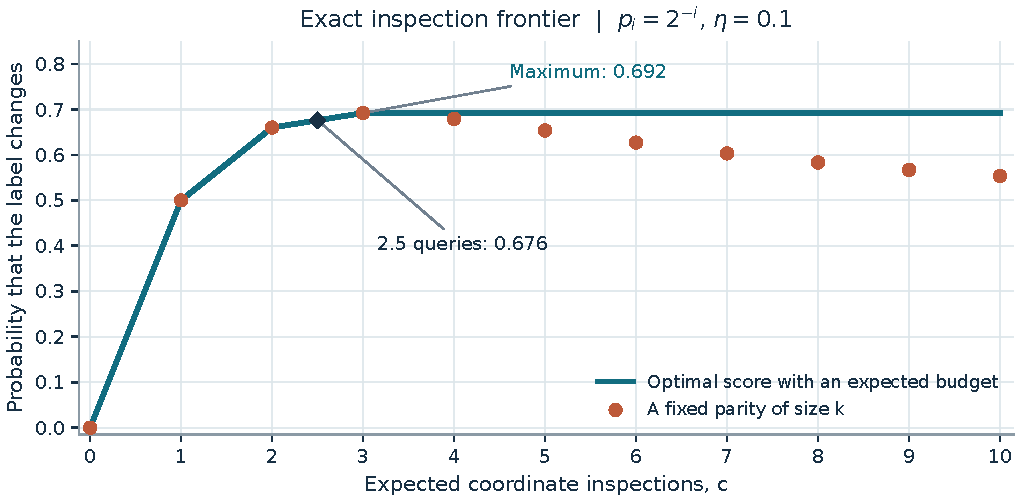
\includegraphics[width=.94\textwidth]{figures/inspection_frontier.pdf}
 \caption{The exact inspection frontier for infinite challenge weights
 \(p_i=2^{-i}\) at \(\eta=0.1\). Dots show the scores of fixed parity sizes;
 the solid line is the optimum under an expected query budget. After the
 third bit, more inspection is unhelpful.}
 \label{np:fig:budget}
\end{figure}

\begin{proposition}[Boundary noise rates]\label{np:prop:boundary}
At \(\eta=0\), the expected-budget optimum is the linear interpolation of
\((k,P_k)\), capped at one in finite dimension. At \(\eta=1/2\), it is
\(\frac12\min(c,1)\).
\end{proposition}
\begin{proof}
At zero noise the slopes of the interpolation are \(p_k\), hence
nonincreasing; the preceding argument applies without a finite saturation
index in countable dimension. At noise \(1/2\), \(X\) and \(Y\) are
independent and
\[
 \Win(f)=\frac{1-(\E f)^2}{2}.
\]
All nonempty characters score \(1/2\), and the empty character scores zero.
Formula~\eqref{np:eq:generalbudget} gives the claim, attained by mixing
the empty and a singleton parity when \(c<1\).
\end{proof}

\begin{remark}[{[write]} Deterministic trees miss the frontier between integers, 5~October 2026]
\label{np:rem:deterministic}
Let \(0<\eta<1/2\), let the weights be strictly decreasing
(\(p_1>p_2>\cdots\)), and let \(0<c<K\) be a non-integer. Then every
labeling \(f\) computed by a deterministic (unrandomized) exact adaptive
procedure with expected cost \(\E Q\le c\) has
\(\Win_{p,\eta}(f)<G(c)\). On a finite cube there are finitely many such
procedures, so the optimum over deterministic trees with an average cost
constraint is strictly below \(G(c)\) for every such \(c\). This sharpens
the distinction drawn after the proof of Theorem~\ref{np:thm:main}; how
far below, and whether the supremum reaches \(G(c)\) on a countable cube,
is question~\ref{np:q:dettrees} of Section~\ref{np:sec:further}.
\end{remark}
\begin{proof}
For finite \(S\) put \(u(S)=\bigl(1+a^{|S|}(2p(S)-1)\bigr)/2\), the score of
\(\chi_S\) (Section~\ref{np:sec:exact}). Since \(a>0\), \(u(S)\) increases
strictly with \(p(S)\), and \(p(S)\le P_{|S|}\) with equality only for
\(S=[|S|]\), because the weights are strictly decreasing. Hence
\(u(S)\le w_{|S|}\), with equality only for prefix sets. Also
\(w_k\le G(k)\) for every \(k\) (equality for \(k\le K\); \(G(k)=w_K\ge
w_k\) for \(k>K\)). With \(\alpha(S)=\widehat f(S)^2\),
Theorem~\ref{np:thm:fourier}, Jensen's inequality for the concave \(G\),
the identity~\eqref{np:eq:influence}, Lemma~\ref{np:lem:query} and the
monotonicity of \(G\) give
\[
 \Win(f)=\sum_S\alpha(S)u(S)\le\sum_S\alpha(S)w_{|S|}
 \le\sum_S\alpha(S)G(|S|)\le G(\mathcal I(f))\le G(c).
\]
Suppose equality held throughout. The first equality forces \(\alpha\) to
live on prefix sets \([k]\). The increments \(w_{k+1}-w_k=a^kd_k/2\) are
positive and strictly decreasing for \(k<K\) (both \(a^k\) and \(d_k>0\)
strictly decrease), and \(G\) is constant on \([K,\infty)\); so \(G\) is
strictly increasing on \([0,K]\) and its slope drops strictly at each
integer \(1,\dots,K\). Equality in \(G(\mathcal I(f))\le G(c)\) with
\(\mathcal I(f)\le c<K\) forces \(\mathcal I(f)=c\). Equality in Jensen's
inequality forces the distribution of \(|S|\) to lie in one interval on
which \(G\) is affine, that is in \([m,m+1]\) with \(m+1\le K\), or in
\([K,\infty)\); its mean \(\mathcal I(f)=c\) is a non-integer below \(K\),
so the interval is \([m,m+1]\) with \(m=\lfloor c\rfloor\), and both
\([m]\) and \([m+1]\) carry positive mass. Thus
\(f=A\chi_{[m]}+B\chi_{[m+1]}=\chi_{[m]}(A+B\chi_{\{m+1\}})\) with
\(AB\ne0\). Evaluating at the two values of \(\chi_{\{m+1\}}\), the Boolean
condition gives \((A+B)^2=(A-B)^2=1\), hence \(AB=0\), a contradiction. So
\(\Win(f)<G(c)\). A finite cube has finitely many deterministic exact
procedures that never repeat a query (repetitions can be cached, as in
Section~\ref{np:sec:rules}), so the maximum over them is attained and is
below \(G(c)\).
\end{proof}

\section{All optimizers, stability, and ties}\label{np:sec:stability}

Put \(\lambda_S=a^{|S|}(1-2p(S))\), and let
\(\lambda_*=-F_K<0\). Define
\[
 \mathcal M=\{S\in\Fin(I):\lambda_S=\lambda_*\}.
\]

\begin{theorem}[Optimizer classification]\label{np:thm:optimizers}
Assume \(0<\eta<1/2\).
A measurable Boolean labeling is optimal exactly when its Fourier
coefficients outside \(\mathcal M\) vanish. The family \(\mathcal M\)
is finite, so every optimum depends on finitely many coordinates, modulo
a null set.

If all weights are strictly decreasing, the only optima are
\(\pm\chi_{[K]}\), together with \(\pm\chi_{[K+1]}\) when the two degrees tie.
\end{theorem}
\begin{proof}
Equality in the spectral average occurs exactly when all its mass is on
least-eigenvalue characters. An optimizing set has an optimizing degree
and maximum mass \(P_k\) at that degree. There are at most two such degrees.
For either one, every coordinate in an optimizing set has weight at least
the positive cutoff weight \(p_k\). Only finitely many coordinates meet
this condition, so \(\mathcal M\) is finite.

Strictly decreasing weights give one optimal set at each optimal degree.
If there are two degrees, an optimal function has the form
\[
 f=\chi_{[K]}(A+B\chi_{\{K+1\}}).
\]
The Boolean condition implies \((A+B)^2=(A-B)^2=1\), hence
\(AB=0\) and \(A^2+B^2=1\). The claimed signed parities are the only
possibilities.
\end{proof}

Equal coordinate weights permit additional Boolean functions in the
optimal eigenspace. This is a genuine exception to a tempting stronger
classification.

\begin{example}[An optimal nonlinear rule]\label{np:ex:nonlinear}
Take
\[
 p=(3/5,1/10,1/10,1/10,1/10),\qquad
 \eta=3/20,\quad a=7/10.
\]
Here \(K=3\). Write \(z_i=(-1)^{x_i}\) and set
\[
 f(x)=\frac{z_1}{2}
 (z_2z_3+z_3z_4+z_4z_5-z_2z_5).
\]
If \(z_2=z_4\), the parenthesized half equals \(z_2z_3\); if
\(z_2=-z_4\), it equals \(z_4z_5\). Thus \(f\) is Boolean.
All four of its Fourier terms use coordinate one and two of the
four tied coordinates, so all are optimizing characters.
Its score is \(6029/10000\), although \(f\) is not a parity.
\end{example}

\begin{theorem}[Quantitative stability]\label{np:thm:stability}
There is a positive gap
\[
 \gamma=\inf_{S\notin\mathcal M}(\lambda_S-\lambda_*)>0.
\]
If \(\Win(f)\ge V-\varepsilon\), then
\begin{equation}\label{np:eq:stability}
 \sum_{S\notin\mathcal M}\widehat f(S)^2
 \le\frac{2\varepsilon}{\gamma}.
\end{equation}
If \(\mathcal M=\{S_*\}\), the distance in probability from a suitably
signed \(\chi_{S_*}\) is at most \(\varepsilon/\gamma\).
The same distance bound holds to one of the signed optimal parities at
a crossover with strictly decreasing weights.
\end{theorem}
\begin{proof}
Large degrees have \(|\lambda_S|\le a^{|S|}\to0\), while
\(\lambda_*<0\), so they are separated from the minimum.
Among the finitely many remaining degrees, the nonoptimal degree
maxima have a positive gap. At an optimal degree, a nonmaximizing
coordinate set has mass separated from \(P_k\): after the finitely
many cutoff ties are accounted for, replacing a selected weight by
a strictly lower available weight loses a fixed positive amount.
This proves \(\gamma>0\).

The energy excess is
\[
 2(V-\Win(f))
 =\sum_S(\lambda_S-\lambda_*)\widehat f(S)^2,
\]
which proves \eqref{np:eq:stability}. In the singleton case, write
\(A=|\widehat f(S_*)|\). The best sign has mismatch probability
\((1-A)/2\le(1-A^2)/2\le\varepsilon/\gamma\).

At a strict-weight crossover put
\(A=\widehat f([K])\), \(B=\widehat f([K+1])\).
The conditional expectation of \(f\chi_{[K]}\) given \(x_{K+1}\) is
\(A+B\chi_{\{K+1\}}\), of absolute value at most one. Thus
\(|A|+|B|\le1\) and
\(\max(|A|,|B|)\ge A^2+B^2\).
The best signed parity mismatch is at most
\((1-A^2-B^2)/2\), giving the same bound.
\end{proof}

The gap depends on the weights and the noise rate. In particular, it can
shrink as \(\eta\downarrow0\). A fixed-noise stability statement does
not by itself give a uniform small-noise conclusion.

\begin{remark}[{[write]} The gap tends to zero on a countable cube, 5~October 2026]
\label{np:rem:gap-shrinks}
Let \(I=\N\), with all \(p_i>0\), and write \(\gamma(\eta)\) and \(K_\eta\)
for the gap of Theorem~\ref{np:thm:stability} and the smallest maximizing
degree of Theorem~\ref{np:thm:main}. Then
\(0<\gamma(\eta)<2p_{K_\eta}\) for every \(0<\eta<1/2\), and
\(\gamma(\eta)\to0\) as \(\eta\downarrow0\). This proves the source's
``can shrink'' for every such weight sequence: no positive lower bound for
the gap holds uniformly in small \(\eta\). (On a finite cube the write
makes no claim.)
\end{remark}
\begin{proof}
Write \(K=K_\eta\). Since \(F_0=-1\) and the maximum of \(F_k\) is positive,
\(K\ge1\); and \(\lambda_*=-F_K=a^K(1-2P_K)=\lambda_{[K]}\). Because
\(p_j\to0\) and \(p_K>0\), some \(j>K\) has \(p_j<p_K\). Put
\(S=[K-1]\cup\{j\}\) (so \(S=\{j\}\) when \(K=1\)). Then \(|S|=K\),
\(p(S)=P_{K-1}+p_j\), and
\[
 \lambda_S-\lambda_*
 =a^K\bigl[(1-2P_{K-1}-2p_j)-(1-2P_K)\bigr]
 =2a^K(p_K-p_j)\in(0,2p_K).
\]
In particular \(\lambda_S\ne\lambda_*\), so \(S\notin\mathcal M\) and
\(\gamma(\eta)\le\lambda_S-\lambda_*<2p_K\); positivity is
Theorem~\ref{np:thm:stability}.

It remains to show \(K_\eta\to\infty\). Fix \(m\). As \(\eta\downarrow0\),
\(F_k=(1-2\eta)^kb_k\to b_k\) for each of the finitely many
\(k\le m+1\), and \(b_{m+1}>b_k\) for \(k\le m\) because \(b_k=2P_k-1\)
strictly increases (all \(p_i>0\)). Hence for all sufficiently small
\(\eta\), \(F_{m+1}>\max_{k\le m}F_k\), so no \(k\le m\) maximizes and
\(K_\eta>m\). Since \(p_k\to0\), \(2p_{K_\eta}\to0\).
\end{proof}

\section{The infinite limit and escape of finite information}
\label{np:sec:infinite}

\begin{theorem}[A supremum without a measurable maximizer]
\label{np:thm:zero}
Suppose infinitely many \(p_i\) are positive. At zero noise,
\[
 \sup_{f\ \mathrm{measurable}}\Win_{p,0}(f)=1,
 \qquad \Win_{p,0}(f)<1\text{ for every such }f.
\]
\end{theorem}
\begin{proof}
Every finite character has score \(p(S)<1\), and
Theorem~\ref{np:thm:fourier} expresses each measurable score as a
probability-weighted average of these strictly smaller numbers.
Such an average is strictly below one. The prefix parities have
scores \(P_k\to1\), proving the supremum.
\end{proof}

\begin{theorem}[Every near-perfect sequence loses its finite-coordinate limit]
\label{np:thm:escape}
For a measurable Boolean \(f\), write
\(\epsilon(f)=1-\Win_{p,0}(f)\). Then
\begin{equation}\label{np:eq:escape}
 \left\|\E[f\mid X_1,\ldots,X_m]\right\|_2^2
 \le\frac{\epsilon(f)}{1-P_m}.
\end{equation}
If \(\Win_{p,0}(f_j)\to1\), then \(f_j\) converges weakly to zero in
\(L^2(\mu)\). No subsequence converges in measure to a Boolean function.
\end{theorem}
\begin{proof}
The spectral identity gives
\[
 \epsilon(f)=\sum_S(1-p(S))\widehat f(S)^2.
\]
For \(S\subseteq[m]\), \(1-p(S)\ge1-P_m\). Summing these coefficients
proves \eqref{np:eq:escape}. Each fixed finite-coordinate projection
therefore tends to zero, and density of cylinder functions plus
\(\|f_j\|_2=1\) proves weak convergence.

If a subsequence converged in measure to a Boolean \(g\), boundedness
would give \(L^2\) convergence: for any \(\delta>0\),
\[
 \E|f_j-g|^2\le\delta^2+
 4\Pbb(|f_j-g|>\delta)\longrightarrow\delta^2.
\]
Letting \(\delta\downarrow0\) gives a strong limit \(g\), necessarily
also the weak limit zero, contradicting \(|g|=1\).
\end{proof}

This is stronger than observing that one particular sequence of parities
fails to converge. Any sequence of increasingly successful measurable
labels must lose its mass from each fixed finite-coordinate Fourier
space. The obstruction concerns attainment and limits, even though every
desired score below one is accessible by a finite rule.

\begin{proposition}[Quantitative finite approximation]
\label{np:prop:truncation}
For \(0\le\eta<1/2\), define the \(n\)-coordinate challenge distribution
\(p_i^{(n)}=p_i/P_n\), \(i\le n\), and let \(V_n\) be its optimum.
Let \(V_\infty\) denote the infinite measurable supremum.
Then
\[
 V_n\downarrow V_\infty,\qquad
 0\le V_n-V_\infty\le1-P_n.
\]
\end{proposition}
\begin{proof}
The finite candidate at degree \(k\le n\) is
\[
 \frac{1+a^k(2P_k/P_n-1)}2.
\]
For fixed \(k\), it decreases as \(n\) increases. The new candidate
at \(k=n+1\) has advantage \(a^{n+1}\), bounded by the old full-parity
advantage \(a^n\). Hence \(V_n\) decreases.
Every infinite candidate with \(k\le n\) is bounded by the corresponding
finite one, and every \(k>n\) has advantage at most \(a^k\le a^n\).
Thus \(V_n\ge V_\infty\).
Finally each finite candidate exceeds its infinite counterpart by
\[
 a^kP_k(P_n^{-1}-1)\le1-P_n.
\]
Take the maximum to get the upper error bound.
\end{proof}

At zero noise all \(V_n\) equal one, but the infinite supremum is
unattained. At fixed positive noise, Theorem~\ref{np:thm:main}
supplies an actual finite measurable optimizer. These statements separate
numerical convergence of optimal values from convergence or existence
of optimizing rules.


\section{Choice, measurability, and summable noise}
\label{np:found:section}

The distinction between a finite cube and the full space
$\cX=\{0,1\}^{\N}$ involves both probability and choice.  In this section all
product measures are completed.  We retain $p_i>0$ and $\sum_i p_i=1$, write
$p(S)=\sum_{i\in S}p_i$, and take labels with values in $\{-1,1\}$.
The fair product measure on $\cX$ is denoted by $\mu$.

\subsection{The classical parity principle}

Two points $x,y\in\cX$ are $E_0$-equivalent if they differ in finitely many
coordinates.  They are $E_{\mathrm{ev}}$-equivalent if that difference is
finite and has even cardinality.  A \emph{total parity label} is a function
$f:\cX\to\{-1,1\}$ satisfying
\begin{equation}
 f(x\oplus e_i)=-f(x)\qquad(x\in\cX,\ i\in\N).
 \label{np:found:parity}
\end{equation}
Repeated application gives the corresponding identity for every finite
set of flipped coordinates.

\begin{proposition}[Classical parity construction]
\label{np:found:choice}
The axiom of choice implies the existence of a total parity label.
More precisely, over ZF its existence is equivalent to the following
restricted choice statement: from each pair of $E_{\mathrm{ev}}$-classes
contained in a single $E_0$-class, one can select one member of that pair.
\end{proposition}

\begin{proof}
Each $E_0$-class splits into exactly two $E_{\mathrm{ev}}$-classes: a
one-coordinate flip exchanges them, and the parity of a finite difference
determines to which one a point belongs.  Selecting one of these two classes
and assigning it the value $1$, with value $-1$ on the other, gives
\eqref{np:found:parity}.  Conversely, a total parity label is constant on
each $E_{\mathrm{ev}}$-class and takes opposite values on the two classes
inside any $E_0$-class, so its $1$-class supplies the selection.

For the usual construction from full choice, select a representative $r_C$
of each $E_0$-class $C$ and put
\[
 f(x)=(-1)^{|\operatorname{supp}(x\oplus r_C)|},\qquad x\in C.
\]
The support in this expression is finite.  Flipping one coordinate changes
its cardinality by one modulo two.
\end{proof}

These constructions and the equivalence with the optimal sequential
infinite hat strategy are classical; see Geschke, Lubarsky, and
Rahn~\cite{glr}.  The restricted choice statement above must not be replaced
by full choice, or by choice for arbitrary families of pairs.  Nor should
the sufficient constructions using a nonprincipal ultrafilter or an
$E_0$-transversal be mistaken for necessary conditions.  Serafin proved,
relative to the consistency of an inaccessible cardinal, that a model of
ZF+DC can contain a parity function while containing neither a nonprincipal
ultrafilter on $\N$ nor an $E_0$-transversal~\cite{serafin}.  This answers
the corresponding question in the earlier paper negatively.

\begin{proposition}[Classical regularity obstruction]
\label{np:found:regularity}
In the graph on $\cX$ whose edges join points differing in one coordinate,
every $\mu$-measurable independent set has measure zero, and every
independent set with the Baire property is meager.  Consequently the graph
has no countable proper measurable coloring and no countable proper
Baire-measurable coloring.  In particular, no total parity label is
measurable or Baire-measurable.
\end{proposition}

\begin{proof}
Suppose that a measurable independent set $A$ has positive measure.
Approximation by finite-coordinate cylinders, or martingale convergence,
gives a nonempty cylinder $C$ with
$\mu(A\cap C)>\mu(C)/2$.  Choose $i$ beyond the coordinates specified by
$C$.  The map $x\mapsto x\oplus e_i$ preserves $C$ and its measure.
Therefore $A\cap C$ and its image intersect, producing an edge with both
endpoints in $A$, a contradiction.

If an independent set $A$ has the Baire property and is nonmeager, there
is a nonempty cylinder $C$ on which it is comeager.  A coordinate flip
beyond the specified prefix maps $C$ homeomorphically to itself.  The two
comeager sets $A\cap C$ and its image intersect, giving the same
contradiction.  Finally, countably many null sets cannot cover $\cX$, and
countably many meager sets cannot cover the nonempty Baire space $\cX$.
Apply these statements to the color classes.
\end{proof}

This stronger chromatic formulation is also classical; Conley and
Miller explicitly record the example~\cite{conleymiller}.  Together with
Theorem~\ref{np:thm:zero}, it displays two different facts: measurable
zero-noise scores can approach one arbitrarily closely, whereas no
countable regular proper coloring exists.

\subsection{Measurable labels and measurable success events}

A nonmeasurable label need not make every question about it
nonmeasurable.  At zero noise, a total parity label succeeds for every
$(x,j)$, so its success event is the whole sample space.  For later use,
we therefore distinguish the class $\mathcal L_{\mu}$ of $\mu$-measurable
labels from the class $\mathcal L_{\mathrm{evt}}$ of arbitrary total labels for which
\begin{equation}
 \{(x,j,z):f(x)\ne f(x\oplus e_j\oplus z)\}
 \label{np:found:success-event}
\end{equation}
is measurable for the completed joint experiment.  Its probability
$\Win(f)$ is defined for $f\in\mathcal L_{\mathrm{evt}}$.  Since the perturbed
configuration also has fair product distribution, $\mathcal L_{\mu}\subseteq
\mathcal L_{\mathrm{evt}}$.  No integral of a nonmeasurable label alone is intended.

\begin{proposition}[Parity under a biased product measure]
\label{np:found:biased}
Let $f$ be any total parity label, and let $\nu_q$ be the product measure
with independent Bernoulli$(q_i)$ coordinates, where $0<q_i<1$.  Then
$f$ is measurable for the completion of $\nu_q$ if and only if
\begin{equation}
 \sum_{i=1}^{\infty}\min(q_i,1-q_i)<\infty.
 \label{np:found:biased-threshold}
\end{equation}
\end{proposition}

\begin{proof}
Choose the modal sequence $b$ by setting $b_i=1$ when $q_i>1/2$ and
$b_i=0$ otherwise.  If \eqref{np:found:biased-threshold} holds, the first
Borel--Cantelli lemma says that $\nu_q$-almost every $x$ differs from $b$
in finitely many coordinates.  The class $[b]_{E_0}$ is countable and
Borel, and on it
\[
 f(x)=f(b)(-1)^{|\operatorname{supp}(x\oplus b)|}.
\]
This restriction has a Borel extension to $\cX$, for example by assigning
the value $1$ outside the class.  The extension agrees with $f$ almost
everywhere, proving measurability for the completed measure.

For the converse, translation by $b$ preserves the parity property and
replaces $q_i$ by $\min(q_i,1-q_i)$.  Thus suppose that
$0<q_i\le 1/2$, $\sum_i q_i=\infty$, and $f$ is measurable.  Fix a
cylinder $C$ depending on the first $n$ coordinates.  Integrating first
over the coordinates $n<i\le m$ and using the parity identity gives
\begin{equation}
 \left|\int_C f\,d\nu_q\right|
 \le \nu_q(C)\prod_{i=n+1}^{m}(1-2q_i).
 \label{np:found:block-bound}
\end{equation}
Indeed, for fixed coordinates outside this block, the label on the
block is its finite parity times a sign independent of the block.
All finite block atoms have positive probability, so the necessary
sections of a completed-measurable function are measurable almost
everywhere, and finite Fubini applies.

Every tail sum of the $q_i$ diverges.  The product in
\eqref{np:found:block-bound} therefore tends to zero, using
$1-2q_i\le \exp(-2q_i)$, with the conclusion immediate if a factor
vanishes.  All cylinder integrals are zero.  It follows that
$\E_{\nu_q}[f\mid x_1,\ldots,x_n]=0$ for every $n$.
Martingale convergence now gives $f=0$ almost surely, contradicting
$|f|=1$.
\end{proof}

\begin{corollary}[Homogeneous noise excludes total parity events]
\label{np:found:homogeneous-event}
If $0<\eta<1$ and the noise coordinates are independent
Bernoulli$(\eta)$ variables, no total parity label belongs to
$\mathcal L_{\mathrm{evt}}$.
\end{corollary}

\begin{proof}
Suppose that \eqref{np:found:success-event} is measurable.  Fix $j$ with
$p_j>0$.  Fubini implies that for $\mu$-almost every $x$ its section as
a function of $z$ is measurable for the completed noise law.  However,
for every fixed $x,j$ the sign
\[
 z\longmapsto f(x)f(x\oplus e_j\oplus z)
\]
is itself a total parity label on the noise space.  Proposition
\ref{np:found:biased} rules out its measurability, since
$\sum_i\min(\eta,1-\eta)=\infty$.  The success indicator determines
this sign, so the same obstruction applies to the event section.
\end{proof}

Thus an arbitrary total parity cannot simply be inserted into the
positive homogeneous-noise objective.  The obstruction concerns the
success event itself.  The next result shows exactly how summable noise
changes this conclusion.

\subsection{An exact classification for summable heterogeneous noise}

Assume for the remainder of this section that
\begin{equation}
 0\le\eta_i<\tfrac12,
 \qquad \sum_i\eta_i<\infty,
 \qquad a_i=1-2\eta_i.
 \label{np:found:summable-assumptions}
\end{equation}
For every subset $S\subseteq\N$, including infinite subsets, define
\begin{equation}
 a(S)=\prod_{i\in S}a_i,
 \qquad F(S)=(2p(S)-1)a(S),
 \qquad A=a(\N).
 \label{np:found:compact-objective}
\end{equation}
All these products are positive: only finitely many $\eta_i$ can be
bounded away from zero, their factors are nonzero, and the remaining
logarithms have absolutely summable magnitude.

\begin{theorem}[Summable-noise optimization]
\label{np:found:summable-theorem}
Under \eqref{np:found:summable-assumptions}, let
\[
 M=\max_{S\subseteq\N}F(S),\qquad V=\frac{1+M}{2}.
\]
Then the maximum defining $M$ exists, and the following hold.
\begin{enumerate}
 \item $M=\sup\{F(S):S\subseteq\N\text{ is finite}\}$.
 \item $\sup_{f\in\mathcal L_{\mu}}\Win(f)=V$.
 \item A measurable label attains $V$ if and only if at least one
 maximizing subset $S$ is finite.
 \item In ZFC, $\max_{f\in\mathcal L_{\mathrm{evt}}}\Win(f)=V$; a maximizing
 label can be constructed from a maximizing subset $S$.
\end{enumerate}
\end{theorem}

\begin{proof}
\emph{Compactness of the scalar problem.}
Identify subsets of $\N$ with Cantor space.  Write
$S_n=S\cap\{1,\ldots,n\}$, $P_n=\sum_{i\le n}p_i$, and
$R_n=\sum_{i>n}\eta_i$.  The elementary inequality
$1-\prod_j(1-t_j)\le\sum_jt_j$ gives
\[
 0\le a(S_n)-a(S)\le 2R_n.
\]
Consequently
\begin{equation}
 |F(S)-F(S_n)|\le 2(1-P_n)+2R_n,
 \label{np:found:uniform-truncation}
\end{equation}
uniformly in $S$.  Each truncated function is continuous, so $F$ is
continuous.  Compactness supplies a maximizer; finite subsets are dense,
proving the first assertion.

\emph{Measurable labels.}
The Walsh calculation of Theorem~\ref{np:thm:fourier} applies with
$a(S)$ in place of the homogeneous factor.  More explicitly, for each
finite $S$ the character
$\chi_S(x)=(-1)^{\sum_{i\in S}x_i}$ has channel eigenvalue
$a(S)(1-2p(S))$.  The finite Walsh characters form an orthonormal basis
of $L^2(\mu)$, and hence every measurable label satisfies
\begin{equation}
 2\Win(f)-1
 =\sum_{S\text{ finite}}F(S)\widehat f(S)^2,
 \qquad
 \sum_{S\text{ finite}}\widehat f(S)^2=1.
 \label{np:found:anisotropic-fourier}
\end{equation}
This bounds its score by $V$, and finite characters approximate $V$ by
the first assertion.  If a finite subset maximizes, its character attains
$V$.  Conversely, if every finite $S$ has $F(S)<M$, the right side of
\eqref{np:found:anisotropic-fourier} is a countable probability-weighted
average of numbers strictly smaller than $M$ and is itself strictly
smaller than $M$.  This proves the second and third assertions.

\emph{Construction for an arbitrary maximizing subset.}
Choose representatives $r_C$ of the $E_0$-classes and, for a fixed
$S\subseteq\N$, set
\begin{equation}
 f_S(x)=(-1)^{|S\cap\operatorname{supp}(x\oplus r_C)|},
 \qquad x\in C.
 \label{np:found:generalized-parity}
\end{equation}
For any vector $u$ of finite support this satisfies
\begin{equation}
 f_S(x)f_S(x\oplus u)=(-1)^{|S\cap\operatorname{supp}(u)|}.
 \label{np:found:finite-cocycle}
\end{equation}
By Borel--Cantelli, $Z$ has finite support almost surely.  Therefore,
almost surely,
\[
 f_S(X)f_S(X\oplus e_J\oplus Z)
 =(-1)^{\mathbf1_{\{J\in S\}}+|S\cap\operatorname{supp}(Z)|}.
\]
The success event thus agrees almost surely with an event depending
only on $(J,Z)$ and is measurable for the completed joint law.
Independence, followed by bounded convergence for finite noise
truncations, gives correlation $(1-2p(S))a(S)$ and score
$(1+F(S))/2$.  A maximizing $S$ consequently realizes $V$ in
$\mathcal L_{\mathrm{evt}}$.

\emph{Upper bound for arbitrary labels with measurable events.}
This step cannot use the Fourier coefficients of $f$, since they need
not exist.  Let $f\in\mathcal L_{\mathrm{evt}}$ and condition the experiment on
\[
 B_n=\{J\le n,\ Z_i=0\text{ for all }i>n\},
 \qquad
 \alpha_n=\Pbb(B_n)=P_n\prod_{i>n}(1-\eta_i).
\]
Summability gives $\alpha_n\to1$.  Conditional on $B_n$, the challenge
weights are $p_i/P_n$ for $i\le n$, and the first $n$ noise coordinates
retain their original independent distributions.

This conditional experiment has only finitely many pairs $(j,z)$.
For each pair of positive conditional probability, the corresponding
success section
\[
 h_{j,z}(x)=\mathbf1_{\{f(x)\ne f(x\oplus e_j\oplus z)\}}
\]
is $\mu$-measurable.  Indeed, summable noise is supported on the
countable set of finite-support vectors; every pair used here is a
positive atom of the $(J,Z)$ law, so completed joint measurability
implies measurability of that section.  Pairs of probability zero do
not enter the conditional average.

Average the conditional success function over the $2^n$ translations
$x\mapsto x\oplus u$ supported on $\{1,\ldots,n\}$.  Translation
invariance of $\mu$ preserves its integral.  At every fixed $x$, however,
the resulting orbit average is precisely the finite-cube score of the
Boolean function $u\mapsto f(x\oplus u)$.  This is a finite function
irrespective of the regularity of $f$.  The finite Fourier theorem
bounds the orbit average pointwise by
\[
 W_n=\frac12\left[1+
 \max_{S\subseteq\{1,\ldots,n\}}
 a(S)\left(\frac{2p(S)}{P_n}-1\right)\right].
\]
For every candidate in this maximum, its conditional score differs
from its original score by
\[
 a(S)p(S)\left(\frac1{P_n}-1\right)\le 1-P_n.
\]
Thus $W_n\le V+1-P_n$, and the unconditional score satisfies
\[
 \Win(f)\le\alpha_n W_n+(1-\alpha_n).
\]
Taking $n\to\infty$ proves $\Win(f)\le V$.  Combined with the
construction above, this completes the proof.
\end{proof}

The theorem identifies the same numerical value in the two regularity
classes, but attainment can differ.  Its compact parameter space consists
of arbitrary subsets of coordinates.  The Fourier modes available to a
measurable label are indexed by finite subsets.  This is the source of the
attainment criterion, rather than a failure of compactness of the scalar
objective.

\subsection{Exactly when full infinite parity is optimal}

\begin{theorem}[Full-parity criterion]
\label{np:found:full-parity}
Under \eqref{np:found:summable-assumptions}, the subset $S=\N$
maximizes $F$ if and only if
\begin{equation}
 \eta_i\le p_i\qquad\text{for every }i.
 \label{np:found:full-parity-condition}
\end{equation}
When this condition holds, the maximizing subsets are exactly
\[
 \N\quad\text{and}\quad
 \N\setminus\{j\}\ \text{for those }j\text{ with }\eta_j=p_j.
\]
Consequently the measurable-label supremum is $(1+A)/2$ and is
unattained, whereas a total parity label attains it in $\mathcal L_{\mathrm{evt}}$.
\end{theorem}

\begin{proof}
Deleting a single coordinate gives
\begin{equation}
 F(\N\setminus\{j\})-F(\N)
 =\frac{2A}{a_j}(\eta_j-p_j).
 \label{np:found:deletion-test}
\end{equation}
Thus optimality of $\N$ requires
\eqref{np:found:full-parity-condition}.

Conversely, for any $S\subseteq\N$ and $j\notin S$, direct algebra
gives
\begin{align}
 F(S\cup\{j\})-F(S)
 &=2a(S)\left[(p_j-\eta_j)
 +2\eta_j p\bigl(\N\setminus(S\cup\{j\})\bigr)\right].
 \label{np:found:inclusion-test}
\end{align}
Under \eqref{np:found:full-parity-condition} this is nonnegative.
Adjoin the omitted coordinates successively and use continuity of $F$
to obtain $F(S)\le F(\N)=A$.

If at least two coordinates are omitted, choose any omitted $j$.
When $p_j>\eta_j$, the first term in the brackets of
\eqref{np:found:inclusion-test} is positive.  When
$p_j=\eta_j$, their common value is positive, and the remaining
omitted coordinate has positive challenge mass, making the second
term positive.  Such an $S$ therefore cannot maximize.  A single
omission ties exactly when $\eta_j=p_j$, by
\eqref{np:found:deletion-test}.  This proves the stated classification.
All of these maximizing sets are infinite, so the attainment claims
follow from Theorem~\ref{np:found:summable-theorem}.
\end{proof}

\begin{remark}[Positive noise at every coordinate without a measurable optimizer]
\label{np:found:dyadic-example}
For any positive probability sequence $p$, set
\[
 \eta_i=\frac{p_i^2}{2},\qquad a_i=1-p_i^2.
\]
Then $0<\eta_i<p_i$ and $\sum_i\eta_i<\infty$.
The unique maximizing subset is $\N$, and the common optimal value is
\[
 V=\frac12\left(1+\prod_{i=1}^{\infty}(1-p_i^2)\right).
\]
Every finite parity is strictly suboptimal, and
\eqref{np:found:anisotropic-fourier} excludes every other measurable
optimizer as well.  For the concrete choice $p_i=2^{-i}$,
\[
 \prod_{i=1}^{\infty}(1-4^{-i})
 \approx0.6885375371203397,
 \qquad
 V\approx0.8442687685601699.
\]
A total choice-based parity label attains this value with a measurable
success event.  The strict inequalities $\eta_i>0$ at every coordinate
therefore do not suffice for the finite optimizer conclusion proved
for homogeneous noise.
\end{remark}

The probabilistic distinction is concrete.  Homogeneous positive noise
flips infinitely many coordinates almost surely and takes the experiment
outside the finite-difference relation.  Summable noise flips only
finitely many coordinates almost surely, so the parity identities remain
valid on almost every experiment.  Proposition~\ref{np:found:biased}
and Theorem~\ref{np:found:summable-theorem} make these two statements
precise without assigning probabilities to nonmeasurable events.

\section{Small-noise laws and finite-size transitions}
\label{np:asym:section}

The exact spectral solution permits a more quantitative question: how many
coordinates should a successful rule retain as the noise decreases, and how
quickly does its failure probability vanish?  The answers depend strongly on
the tail of the distinguished-coordinate distribution.  Exponential tails
produce logarithmic degrees and a periodic second-order correction; power
law tails produce fractional powers of the noise.  A finite uniform model
has a separate saturation transition.

Throughout this section $0<\eta<1/2$ and the weights are arranged in nonincreasing order.
We retain the notation
\[
 a=1-2\eta,\qquad t_k=1-P_k,\qquad b_k=1-2t_k,
 \qquad F_k=a^k b_k,\qquad w_k=\frac{1+F_k}{2},
\]
and write
\[
 V(\eta)=\max_k w_k,\qquad L(\eta)=1-V(\eta).
\]
The symbol $k_\eta$ denotes any specifically chosen maximizing degree;
it need not be the smallest maximizing degree $K_\eta=K(p,\eta)$ from Theorem~\ref{np:thm:main}.
An elementary identity controls every degree transition:
\begin{equation}
 F_k-F_{k-1}=2a^{k-1}(p_k-\eta b_k).
 \label{np:asym:increment}
\end{equation}
On the range $b_k>0$, the ratios $h_k=p_k/b_k$ strictly decrease.
Consequently a maximizing degree satisfies
\begin{equation}
 \frac{p_{k+1}}{b_{k+1}}\leq\eta\leq\frac{p_k}{b_k},
 \label{np:asym:crossover}
\end{equation}
where the left endpoint is zero at the last coordinate of a finite model.
At a crossover two adjacent degrees may be optimal.  These statements
concern degrees; ties between coordinate weights or within an extremal
Fourier eigenspace can allow additional maximizing functions.

\subsection{Uniform finite models and the saturation transition}
\label{np:asym:uniform}

\begin{proposition}[Uniform weights]
\label{np:asym:uniform-exact}
For $p_1=\cdots=p_n=1/n$, one maximizing degree is
\begin{equation}
 k_\eta=\min\left\{n,
       \left\lfloor\frac{n+\eta^{-1}}2\right\rfloor\right\},
 \qquad
 V_n(\eta)=\frac12\left[1+(1-2\eta)^{k_\eta}
                              \frac{2k_\eta-n}{n}\right].
 \label{np:asym:uniform-formula}
\end{equation}
If $(n+\eta^{-1})/2$ is an integer at most $n$, that integer and its
predecessor tie.  Otherwise the maximizing cardinality is unique.
In particular, all $n$ coordinates are optimal whenever $\eta\leq1/n$.
\end{proposition}

\begin{proof}
For $k>n/2$ one has $b_k=(2k-n)/n$ and
$h_k=1/(2k-n)$.  Inserting this into
\eqref{np:asym:crossover} gives the formula and the tie rule.
The last degree becomes optimal at $h_n=1/n$.
\end{proof}

\begin{theorem}[A finite-size transition]
\label{np:asym:uniform-limit}
Fix $c>0$ and let $\eta=c/n$.  As $n\to\infty$,
\begin{equation}
 \frac{k_\eta}{n}\longrightarrow
 s(c)=
 \begin{cases}
  1,&0<c\leq1,\\[1mm]
  (1+c^{-1})/2,&c\geq1,
 \end{cases}
 \label{np:asym:uniform-degree-limit}
\end{equation}
and
\begin{equation}
 2V_n(c/n)-1=\mathcal A(c)+O_c(n^{-1}),\qquad
 \mathcal A(c)=
 \begin{cases}
  e^{-2c},&0<c\leq1,\\[1mm]
  c^{-1}e^{-c-1},&c\geq1.
 \end{cases}
 \label{np:asym:uniform-score-limit}
\end{equation}
The function $\mathcal A$ is continuously differentiable at $c=1$, but its
one-sided second derivatives there are $4e^{-2}$ and $5e^{-2}$.
\end{theorem}

\begin{proof}
The exact formula gives $k_\eta=ns(c)+O(1)$, while
$\log(1-2c/n)=-2c/n+O_c(n^{-2})$.
Thus the limiting advantage is $e^{-2cs}(2s-1)$ evaluated at $s=s(c)$.
Equivalently, maximizing this expression on $1/2\leq s\leq1$ gives the
unconstrained critical point $s=(1+c^{-1})/2$; it first enters the
admissible interval at $c=1$.  Direct differentiation proves the final
assertion.
\end{proof}

For fixed $\eta>0$, in contrast, $V_n(\eta)\to1/2$ exponentially.
Writing $k=n/2+u$, the exact advantage, once the upper endpoint is
inactive, is
\[
 2V_n(\eta)-1=\frac{2a^{n/2}}{n}
       \max_{u\in\Lambda_n,\ u>0}u a^u,
 \qquad
 \Lambda_n=
 \begin{cases}\mathbb Z,&n\text{ even},\\
               \mathbb Z+\tfrac12,&n\text{ odd}.
 \end{cases}
\]
The prefactor therefore remembers the parity of $n$.
Neither limit constitutes a countably infinite uniform model:
there is no uniform probability distribution on a countably infinite
coordinate set.


\begin{figure}[tb]
 \centering
 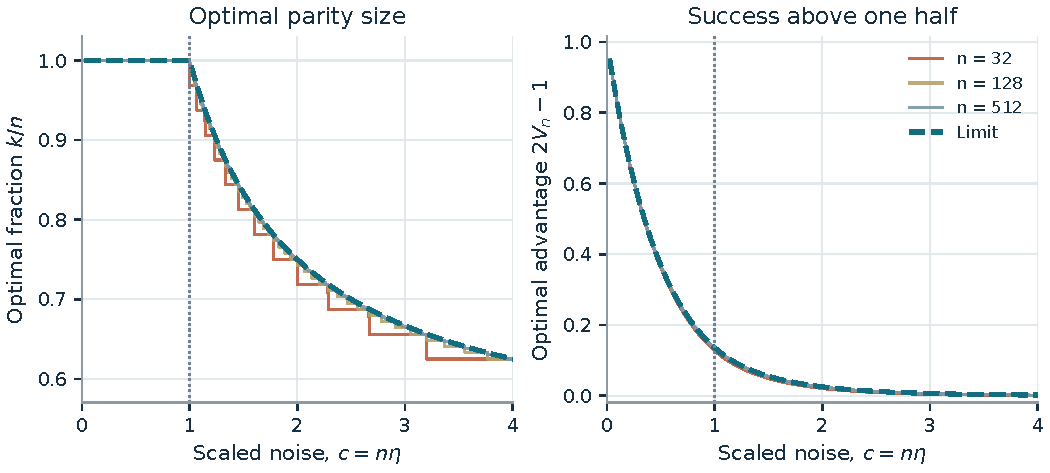
\includegraphics[width=\textwidth]{figures/uniform_transition.pdf}
 \caption{Uniform finite challenge distributions under the scaling
 $\eta=c/n$. Left: the fraction of coordinates in an optimal parity.
 Right: the optimal advantage $2V_n-1$. Curves for finite $n$ approach
 the limits in Theorem~\ref{np:asym:uniform-limit}; $c=1$ is the
 saturation threshold.}
 \label{np:fig:uniform}
\end{figure}

\FloatBarrier
\subsection{Geometric tails and a periodic second term}
\label{np:asym:geometric}

\begin{theorem}[Geometric weights]
\label{np:asym:geometric-theorem}
Suppose $p_k=(1-r)r^{k-1}$, where $0<r<1$, and put $\ell=-\log r$.
Define
\begin{equation}
 x_\eta=\frac1\ell\log\frac{1-r+2\eta r}{\eta r},
 \qquad u_\eta=\{x_\eta\}.
 \label{np:asym:geometric-root}
\end{equation}
Then $k_\eta=\lfloor x_\eta\rfloor$ is optimal; if $x_\eta$ is an
integer, its predecessor also ties.  In particular,
\[
 V(\eta)=\frac12\left[1+(1-2\eta)^{\lfloor x_\eta\rfloor}
                           \bigl(1-2r^{\lfloor x_\eta\rfloor}\bigr)\right].
\]
As $\eta\downarrow0$,
\begin{equation}
 L(\eta)=\frac{\eta}{\ell}\log\frac1\eta
          +\eta\Phi_r(u_\eta)
          +O_r\!\left(\eta^2\log^2\frac1\eta\right),
 \label{np:asym:geometric-expansion}
\end{equation}
where
\begin{equation}
 \Phi_r(u)=\frac{\log((1-r)/r)}{\ell}
                -u+\frac{r}{1-r}e^{\ell u},\qquad 0\leq u\leq1.
 \label{np:asym:geometric-periodic}
\end{equation}
The endpoint identity $\Phi_r(0)=\Phi_r(1)$ makes $\Phi_r$ a continuous
periodic function.  The error estimate is uniform through degree
crossovers.
\end{theorem}

\begin{proof}
Here $t_k=r^k$ and
\[
 h_k=\frac{(1-r)r^{k-1}}{1-2r^k}.
\]
Solving $h_k=\eta$ for real $k$ gives
\eqref{np:asym:geometric-root}; monotonicity and
\eqref{np:asym:increment} give the exact integer rule.
Set $c_r=\log((1-r)/r)$.  Uniformly in $u_\eta\in[0,1)$,
\begin{align*}
 k_\eta&=\frac{\log(1/\eta)+c_r}{\ell}-u_\eta+O_r(\eta),\\
 r^{k_\eta}
 &=\frac{\eta r}{1-r+2\eta r}e^{\ell u_\eta}
   =\eta\frac{r}{1-r}e^{\ell u_\eta}+O_r(\eta^2).
\end{align*}
Since $k_\eta=O_r(\log(1/\eta))$,
\[
 a^{k_\eta}=1-2\eta k_\eta
                   +O_r\!\left(\eta^2\log^2(1/\eta)\right).
\]
Substitution into $L=(1-a^{k_\eta})/2+a^{k_\eta}r^{k_\eta}$ yields
\eqref{np:asym:geometric-expansion}.  The endpoint identity follows
by direct evaluation.
\end{proof}

Thus $k_\eta\sim\ell^{-1}\log(1/\eta)$ and
$L(\eta)\sim(\eta/\ell)\log(1/\eta)$.
The next coefficient is generally periodic rather than constant.
Because the periodic extension of $\Phi_r$ is Lipschitz, one may replace
$u_\eta$ by
$\{\ell^{-1}\log((1-r)/(\eta r))\}$ in
\eqref{np:asym:geometric-expansion} without changing its error term.


\begin{figure}[tb]
 \centering
 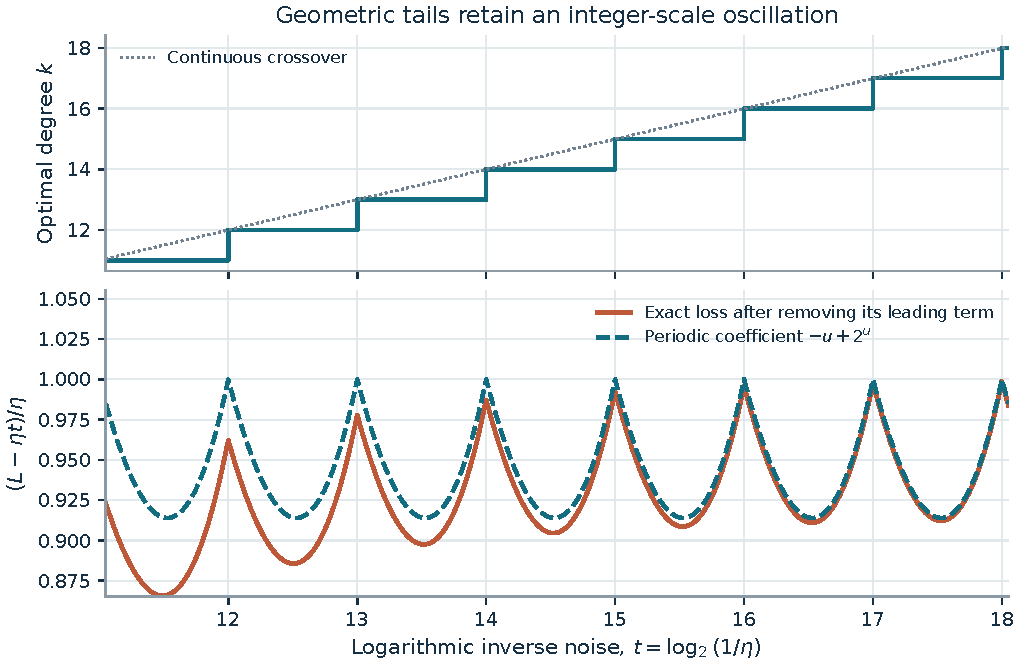
\includegraphics[width=.96\textwidth]{figures/geometric_correction.pdf}
 \caption{For $p_i=2^{-i}$, the optimal degree grows in integer steps
 as $\eta$ decreases. The lower panel removes the leading term from
 the optimal failure probability and displays the periodic correction
 $\Phi_{1/2}(u)=-u+2^u$. The finite-noise residual approaches this
 correction as the error term in Theorem~\ref{np:asym:geometric-theorem}
 decreases.}
 \label{np:fig:geometric}
\end{figure}

\FloatBarrier
\subsection{Regularly varying tails and degree stability}
\label{np:asym:regular-variation}

A positive sequence is regularly varying with index $-\alpha$ if
\[
 \frac{p_{\lfloor tk\rfloor}}{p_k}\longrightarrow t^{-\alpha}
 \quad\text{for each fixed }t>0.
\]
The following result applies to the standing nonincreasing ordering of
the weights.

\begin{theorem}[The power law for optimal failure]
\label{np:asym:regular-theorem}
Suppose $(p_k)$ is regularly varying with index $-\alpha$, where
$\alpha>1$.  For any maximizing degree $k_\eta$,
\begin{equation}
 p_{k_\eta}\sim\eta,\qquad
 t_{k_\eta}\sim\frac{k_\eta p_{k_\eta}}{\alpha-1},\qquad
 L(\eta)\sim\frac{\alpha}{\alpha-1}\eta k_\eta.
 \label{np:asym:regular-laws}
\end{equation}
Moreover, for each $c>0$,
$k_{c\eta}/k_\eta\to c^{-1/\alpha}$.
In particular, if $p_k\sim Ck^{-\alpha}$, then, with
$R=(C/\eta)^{1/\alpha}$,
\begin{equation}
 k_\eta\sim R,\qquad
 L(\eta)\sim\frac{\alpha}{\alpha-1}
            C^{1/\alpha}\eta^{(\alpha-1)/\alpha}.
 \label{np:asym:pure-power-law}
\end{equation}
\end{theorem}

\begin{proof}
We first justify the tail estimate
\begin{equation}
 \frac{t_k}{kp_k}\longrightarrow\int_1^\infty x^{-\alpha}\,dx
                  =\frac1{\alpha-1}.
 \label{np:asym:tail-integral}
\end{equation}
On every compact interval of positive $x$, the ratios
$p_{\lfloor xk\rfloor}/p_k$ converge uniformly: they are nonincreasing
in $x$ and their pointwise limit is continuous.  Riemann sums therefore
give the truncated integral.  To control the remaining tail, choose
$0<\delta<\alpha-1$ and a fixed dilation $q>1$.
Regular variation, with harmless adjustments of integer endpoints,
bounds the contribution of the $j$th block
$[q^jk,q^{j+1}k)$ by a constant times
$q^{j(1-\alpha+\delta)}$.  The resulting geometric series is summable,
uniformly for all sufficiently large $k$, and its tail tends to zero.
This proves \eqref{np:asym:tail-integral}.

The crossover rule implies $k_\eta\to\infty$.
Monotonicity and regular variation also imply
$p_{k+1}/p_k\to1$; hence the two sides of
\eqref{np:asym:crossover} are asymptotically equal to $p_k$.
It follows that $p_{k_\eta}\sim\eta$.
Summability and monotonicity imply $kp_k\to0$, so
$\eta k_\eta\to0$ and
\[
 L(\eta)=\frac{1-a^{k_\eta}}2+a^{k_\eta}t_{k_\eta}
        =\eta k_\eta+t_{k_\eta}
                      +o(\eta k_\eta+t_{k_\eta}).
\]
Together with \eqref{np:asym:tail-integral}, this proves
\eqref{np:asym:regular-laws}.
Finally, regular variation brackets the index at which $p_k$ crosses
$c\eta$ between fixed multiples of $k_\eta$ approaching
$c^{-1/\alpha}$.  This proves the inverse scaling assertion and its
pure-power specialization.
\end{proof}

For example, if
$p_k\sim Ck^{-\alpha}(\log k)^\beta$, then direct inversion gives
\[
 k_\eta\sim C^{1/\alpha}\alpha^{-\beta/\alpha}
       \eta^{-1/\alpha}\bigl(\log(1/\eta)\bigr)^{\beta/\alpha},
\]
and the failure probability is asymptotic to
$\alpha\eta k_\eta/(\alpha-1)$.

\begin{proposition}[The degree-regret profile]
\label{np:asym:regret}
Assume $p_k\sim Ck^{-\alpha}$, and let
$R=(C/\eta)^{1/\alpha}$.  For each fixed $u>0$,
\begin{equation}
 \frac{1-w_{\lfloor uR\rfloor}}{\eta R}
 \longrightarrow
 g_\alpha(u)=u+\frac{u^{1-\alpha}}{\alpha-1}.
 \label{np:asym:regret-profile}
\end{equation}
The convergence is uniform on compact subintervals of $(0,\infty)$.
The unique minimum is $g_\alpha(1)=\alpha/(\alpha-1)$, and
\[
 g_\alpha(1+d)-g_\alpha(1)=\frac\alpha2d^2+O_\alpha(d^3).
\]
Consequently, if a sequence of parity degrees has failure probability
asymptotic to $L(\eta)$, its degree divided by $R$ tends to one.
\end{proposition}

\begin{proof}
For $k=\lfloor uR\rfloor$, expand
$(1-a^k)/2\sim\eta k$ and use
$t_k\sim Ck^{1-\alpha}/(\alpha-1)$.
This proves \eqref{np:asym:regret-profile}; differentiation gives the
minimum and its quadratic expansion.  A degree with $k/R\to0$ has a
tail loss too large on the scale $\eta R$.  A degree with $k/R\to\infty$
has a noise loss too large on that scale, whether or not $\eta k$ tends
to zero.  Every near-optimal sequence is therefore confined to a compact
range of positive $k/R$, where the unique minimum forces $k/R\to1$.
\end{proof}

The Fourier formula extends this conclusion beyond parity rules.
If a Boolean rule has success deficit $o(\eta R)$, then, for every fixed
$\delta>0$, its Fourier mass on sets satisfying
$\lvert |S|/R-1\rvert\geq\delta$ tends to zero.
Indeed, the preceding proof supplies a positive gap of order $\eta R$
outside that degree range, and a set of size $k$ cannot outperform the
$k$ largest weights.  Averaging those gaps with the squared Fourier
coefficients proves the assertion.

\subsection{Exact Zipf weights: an envelope and second-order laws}
\label{np:asym:zipf}

Second-order statements require more than a leading tail equivalence.
We now impose the exact distribution
\[
 p_k=Ck^{-\alpha},\qquad C=\zeta(\alpha)^{-1},\qquad\alpha>1,
\]
and use the scales
\begin{equation}
 R=(C/\eta)^{1/\alpha},\qquad \varepsilon=\eta R.
 \label{np:asym:zipf-scales}
\end{equation}
Both $\varepsilon$ and $R^{-1}$ tend to zero; keeping them distinct
reveals the competition between tail corrections and integer rounding.

\begin{theorem}[A controlled asymptotic envelope]
\label{np:asym:zipf-envelope}
Let $s=s_\alpha(\varepsilon)>1$ solve
\begin{equation}
 s^\alpha-\frac{2\varepsilon}{\alpha-1}s=1,
 \label{np:asym:saddle-equation}
\end{equation}
and put
\begin{equation}
 M_0=s^{-\alpha}e^{-2\varepsilon s},\qquad E_0=\frac{1-M_0}{2}.
 \label{np:asym:envelope-definitions}
\end{equation}
Then
\begin{equation}
 L(\eta)=E_0+\eta M_0\left(\varepsilon s-\frac12\right)
                     +O_\alpha(\eta/R).
 \label{np:asym:envelope}
\end{equation}
In particular,
\begin{equation}
 L(\eta)=\frac{\alpha}{\alpha-1}\varepsilon
       -\frac{\alpha+1}{\alpha-1}\varepsilon^2-\frac\eta2
       +O_\alpha\!\left(\varepsilon^3+\eta\varepsilon+\frac\eta R\right).
 \label{np:asym:zipf-second-order}
\end{equation}
\end{theorem}

\begin{proof}
The root in \eqref{np:asym:saddle-equation} is unique for $s\geq1$.
The implicit-function theorem at $(s,\varepsilon)=(1,0)$ makes it
analytic for small $\varepsilon$.
Extend the tail to real $x>0$ by $T(x)=C\zeta(\alpha,x+1)$.
Euler--Maclaurin, or the Hurwitz zeta expansion in \cite{dlmf}, gives
\begin{equation}
 T(x)=\frac{C}{\alpha-1}x^{1-\alpha}
          -\frac C2x^{-\alpha}
          +\frac{C\alpha}{12}x^{-\alpha-1}
          +O_\alpha(x^{-\alpha-3}).
 \label{np:asym:zipf-tail}
\end{equation}
The half term is negative because the discrete tail begins at $k+1$.

Let $H$ be the large real solution of
$CH^{-\alpha}/(1-2T(H))=\eta$.  Monotonicity makes
$\lfloor H\rfloor$ an optimal degree, with its predecessor also
permitted at an integer tie.  Writing $H=R\rho$, equation
\eqref{np:asym:zipf-tail} gives
\[
 \rho^\alpha-\frac{2\varepsilon}{\alpha-1}\rho
                  =1-\eta+O_\alpha(\eta/R).
\]
Comparison with \eqref{np:asym:saddle-equation} yields
\begin{equation}
 H=Rs-\frac{\varepsilon}{D}
                  +O_\alpha(\eta+\eta\varepsilon),
 \qquad D=\frac\alpha s+2\varepsilon.
 \label{np:asym:rounding-root}
\end{equation}
Here the derivative of the left side at $s$ equals $D$, by the
saddle equation.  Every maximizing integer thus has
$k=Rs+d$ with $|d|\leq1+O_\alpha(\varepsilon)$.

For the evaluation, define the smooth leading loss
\[
 \mathcal L_0(x)=\frac12\left[1-e^{-2\eta x}
          \left(1-\frac{2C}{\alpha-1}x^{1-\alpha}\right)\right].
\]
Its derivative vanishes at $x_0=Rs$, and
$\mathcal L_0(x_0)=E_0$.
Put
\[
 b_0(\rho)=1-\frac{2\varepsilon}{\alpha-1}\rho^{1-\alpha},
 \qquad
 G_0(\rho)=e^{-2\varepsilon\rho}
       \left[\varepsilon\rho b_0(\rho)-\frac12\rho^{-\alpha}\right].
\]
Uniformly for $\rho$ near one, the exact smooth extension
$\mathcal L(x)=(1-a^x(1-2T(x)))/2$ satisfies
\begin{align}
 \mathcal L(R\rho)
  ={}&\mathcal L_0(R\rho)+\eta G_0(\rho)
       +\frac{\alpha\eta}{12R}
                   e^{-2\varepsilon\rho}\rho^{-\alpha-1}
 \nonumber\\
     &\hspace{12mm}
       +O_\alpha(\eta^2\varepsilon+\eta/R^3).
 \label{np:asym:local-expansion}
\end{align}
This follows by substituting \eqref{np:asym:zipf-tail} and
\[
 a^{R\rho}=e^{-2\varepsilon\rho}
              \left[1-2\eta\varepsilon\rho
                         +O_\alpha(\eta^2\varepsilon)\right].
\]
At $\rho=s$, the saddle equation gives $b_0(s)=s^{-\alpha}$,
so $G_0(s)=M_0(\varepsilon s-1/2)$.
Moving from $Rs$ to the maximizing integer changes
$\mathcal L_0$ by $O_\alpha(\eta/R)$, since its first derivative
vanishes and its second derivative is $O_\alpha(\eta/R)$ there.
The other explicit terms have changes of the same or smaller order.
Finally $\eta^2\varepsilon=(\eta/R)\varepsilon^2$.
Equation \eqref{np:asym:envelope} follows.

Expansion of the implicit root gives
\[
 s=1+\frac{2\varepsilon}{\alpha(\alpha-1)}
       +\frac{2(3-\alpha)\varepsilon^2}{\alpha^2(\alpha-1)^2}
       +O_\alpha(\varepsilon^3).
\]
Substituting into \eqref{np:asym:envelope-definitions} yields
\[
 E_0=\frac{\alpha}{\alpha-1}\varepsilon
          -\frac{\alpha+1}{\alpha-1}\varepsilon^2
          +O_\alpha(\varepsilon^3),
 \qquad
 \eta M_0(\varepsilon s-1/2)=-\eta/2+O_\alpha(\eta\varepsilon),
\]
which proves \eqref{np:asym:zipf-second-order}.
\end{proof}

\begin{corollary}[Three second-order regimes]
\label{np:asym:zipf-regimes}
For the exact Zipf distribution,
\begin{align*}
 1<\alpha<2:\quad
 L(\eta)&=\frac{\alpha}{\alpha-1}\varepsilon
           -\frac{\alpha+1}{\alpha-1}\varepsilon^2
           +o(\varepsilon^2),\\[1mm]
 \alpha=2:\quad
 L(\eta)&=2\sqrt{C\eta}-\left(3C+\frac12\right)\eta
                             +O(\eta^{3/2}),
                  \qquad C=\frac6{\pi^2},\\[1mm]
 \alpha>2:\quad
 L(\eta)&=\frac{\alpha}{\alpha-1}\varepsilon-\frac\eta2+o(\eta).
\end{align*}
\end{corollary}

\begin{proof}
Compare $\varepsilon^2=C^{2/\alpha}\eta^{2-2/\alpha}$ with $\eta$
in \eqref{np:asym:zipf-second-order}.  They exchange order at
$\alpha=2$, where both second-order contributions must be retained.
\end{proof}

The quantified formula \eqref{np:asym:zipf-second-order} is convenient
across all exponents.  It should not be read as resolving every displayed
term separately when that term lies below its stated remainder.
The implicit envelope avoids this issue by retaining an analytic function
of $\varepsilon$ without truncating its powers.

\subsection{The Bernoulli correction from integer degree selection}
\label{np:asym:lattice}

The envelope admits a uniform refinement that records the optimal degree's
position in the integer lattice.  Write $B_2(u)=u^2-u+1/6$ for the second
Bernoulli polynomial.

\begin{theorem}[A lattice refinement for exact Zipf weights]
\label{np:asym:lattice-theorem}
With the notation of Theorem~\ref{np:asym:zipf-envelope},
\begin{align}
 L(\eta)={}&E_0+\eta M_0\left(\varepsilon s-\frac12\right)
          +\frac{\alpha\eta}{2R}B_2(\{Rs\})
 \nonumber\\
 &\hspace{8mm}
       +O_\alpha\!\left(\frac\eta R
                                  \left(\varepsilon+\frac1R\right)\right).
 \label{np:asym:lattice-formula}
\end{align}
The estimate holds through every crossover of the maximizing integer.
\end{theorem}

\begin{proof}
Use \eqref{np:asym:local-expansion} with $k=Rs+d$,
where \eqref{np:asym:rounding-root} bounds $d$.
Direct differentiation gives
\[
 \mathcal L_0'(Rs)=0,\qquad
 \mathcal L_0''(Rs)=\frac\eta R M_0
                                    \left(\frac\alpha s+2\varepsilon\right),
 \qquad
 G_0'(s)=M_0\left(\frac\alpha{2s}+2\varepsilon\right).
\]
Taylor expansion therefore makes the contribution of order $\eta/R$
equal to
\[
 \frac\eta R M_0\left[
       \left(\frac\alpha{2s}+\varepsilon\right)d^2
       +\left(\frac\alpha{2s}+2\varepsilon\right)d
       +\frac\alpha{12s}\right].
\]
Since $s=1+O_\alpha(\varepsilon)$ and
$M_0=1+O_\alpha(\varepsilon)$, this is
\[
 \frac{\alpha\eta}{R}
          \left(\frac{d^2+d}{2}+\frac1{12}\right)
                         +O_\alpha(\eta\varepsilon/R).
\]
The remaining Taylor terms are $O_\alpha(\eta/R^2)$, and the
$\eta^2\varepsilon$ remainder in
\eqref{np:asym:local-expansion} is absorbed because it equals
$(\eta/R)\varepsilon^2$.

Let $u=\{Rs\}$.  Away from an $O_\alpha(\varepsilon)$ neighborhood
of an integer, \eqref{np:asym:rounding-root} gives
$k=\lfloor Rs\rfloor$, hence $d=-u$ and
\[
 \frac{d^2+d}{2}+\frac1{12}=\frac12 B_2(u).
\]
Near a crossover, the selected integer may be the adjacent one.
The endpoint identity $B_2(0)=B_2(1)$ bounds the resulting discrepancy
by $O_\alpha(\varepsilon)$, already included in the error.
The same reasoning covers either choice at an exact tie and proves
\eqref{np:asym:lattice-formula}.
\end{proof}

This refinement separates three effects within one rigorously controlled
expression: the analytic tail optimization, the first correction from
Bernoulli noise and the discrete tail, and the oscillation caused by
integer degree selection.  The final oscillation has scale
$\eta/R=C^{-1/\alpha}\eta^{1+1/\alpha}$, whereas its phase follows the
implicitly determined optimum $Rs_\alpha(\varepsilon)$.

\section{A general theorem for finitely supported perturbations}
\label{np:sec:finiteperturb}

The compactness mechanism in Theorem~\ref{np:found:summable-theorem}
depends on finite perturbations occurring almost surely. Independence of
individual noise bits is unnecessary.

\begin{theorem}[Compact optimization for arbitrary finite perturbations]
\label{np:thm:finiteperturb}
Let \(D\) be any random vector in the countable group
\(\bigoplus_{\N}\Ftwo\), independent of \(X\sim\mu\). For every
\(S\subseteq\N\), define
\[
 q(S)=\Pbb\bigl(|S\cap\supp D|\text{ is odd}\bigr).
\]
Then \(q\) is continuous on the compact space \(2^\N\), and
\[
 \sup_{f\ \mu\text{-measurable}}\Pbb(f(X)\ne f(X\oplus D))
 =\max_{S\subseteq\N}q(S).
\]
The measurable supremum is attained exactly when a finite subset maximizes
\(q\). In ZFC the same value is a maximum over arbitrary total labels
whose comparison event is measurable.
\end{theorem}
\begin{proof}
Let \(A_n=\{\supp D\subseteq[n]\}\). Then \(\Pbb(A_n)\to1\), and
\[
 |q(S)-q(S\cap[n])|\le\Pbb(A_n^c)
\]
uniformly in \(S\). Thus \(q\) is a uniform limit of continuous cylinder
functions. Compactness and density of finite subsets show
\(\max_Sq(S)=\sup_{S\text{ finite}}q(S)\). The measurable claims follow
from Theorem~\ref{np:thm:fourier}, including the strict-average argument
when no finite maximizing subset exists.

For an arbitrary total label with measurable comparison event, take \(n\)
sufficiently large that \(\alpha_n=\Pbb(A_n)>0\), and condition on \(A_n\). Every positive-probability \(D\)-section is measurable.
Average these sections over the finite group of translations supported
on \([n]\). Invariance preserves the integral, and each pointwise orbit
average is the score of a finite Boolean function. Its value is bounded
by \(\max_{S\subseteq[n]}\Pbb(|S\cap\supp D|\text{ odd}\mid A_n)\).
Then
\[
 \alpha_n\max_{S\subseteq[n]}\Pbb(|S\cap\supp D|\text{ odd}\mid A_n)
 \le \max_{S\subseteq\N}q(S).
\]
The unconditional score is therefore at most
\(\max_Sq(S)+1-\alpha_n\); pass to the limit.

Finally, for any fixed subset \(S\), the representative construction
\eqref{np:found:generalized-parity} changes sign under a finite
translation \(D\) exactly when \(|S\cap\supp D|\) is odd.
It has a measurable comparison event of probability \(q(S)\).
Choose a maximizing subset.
\end{proof}

\begin{corollary}[One parity function supplies all compact optimizers]
\label{np:cor:uniformchoice}
Suppose one total parity function $h:\cX\to\{-1,1\}$ exists.
It suffices for the arbitrary-label attainment assertion in
Theorem~\ref{np:thm:finiteperturb}, simultaneously for every law of $D$.
\end{corollary}
\begin{proof}
For each $S\subseteq\N$ define
\[
 h_S(x)=h(x\cdot\one_S),
\]
where coordinates outside $S$ are set to zero. A finite flip $u$ changes
$h_S$ by $(-1)^{|S\cap\supp u|}$, so its comparison score is $q(S)$.
The nonempty compact maximizing set of $q$ has a lexicographically least
member: at each coordinate choose zero if that prefix still has a
maximizing extension, and otherwise choose one. Nested compactness gives
a maximizing limit. Apply $h_S$ to this canonically selected subset.
The same $h$ works for all laws; no additional choice of labels is needed.
\end{proof}

This theorem provides a reusable finite--infinite principle. Measurable
labels use finite Walsh characters. Arbitrary componentwise labels can
realize the characters indexed by all subsets of the countable coordinate
set. Passing to the compact space of all subsets can add maximizers
without increasing the supremum. No new independence or choice
equivalence is inferred from this observation.

\section{Exact computations and reproducibility}\label{np:sec:checks}

The archive includes two complementary checks. Neither is used to replace
a proof of an infinite statement.

\subsection{Exhausting all small Boolean rules}

The program \texttt{code/verify\_parity.py} uses only integer and rational
arithmetic. It enumerates every Boolean truth table in dimensions
\(1,2,3,4\), independently constructs the channel's transition
probabilities, and computes the Walsh transform by integer butterflies.
For each rule it compares direct transition scores with the spectral
formula.

It also computes the minimum exact average decision-tree cost by the
dynamic program
\[
 C_n(f)=
 \begin{cases}
 0,& f\text{ constant},\\
 1+\displaystyle\min_{i\in[n]}
 \frac{C_{n-1}(f|_{x_i=0})+C_{n-1}(f|_{x_i=1})}{2},
 & f\text{ nonconstant}.
 \end{cases}
\]
All choices of the first query are examined, so this is the exact optimum
under uniform input, not a heuristic cost. The routine stores
\(2^nC_n(f)\) as an integer.

\begin{center}
\begin{tabular}{@{}rrrr@{}}
\toprule
Dimension&Truth tables&Parameter cases&Rule--parameter pairs\\
\midrule
1&4&8&32\\
2&16&8&128\\
3&256&8&2,048\\
4&65,536&8&524,288\\
\midrule
Total&65,812&&526,496\\
\bottomrule
\end{tabular}
\end{center}

Every listed case passed the following comparisons: direct versus spectral
score, finite optimum versus \(\max_k w_k\), direct versus spectral total
influence, influence versus minimum query cost, and score versus
\(G(C_n(f))\). The checks include boundary noise rates, uniform,
geometric, and concentrated challenge distributions. They also verify
the interpolation construction and exact crossover examples.
The recorded data are in \texttt{data/verification.json}.

\begin{center}
\small
\begin{tabular}{@{}L{.39\textwidth}cc@{}}
\toprule
Example & First optimal degree & Exact optimal score\\
\midrule
\(n=4,\ p_i=1/4,\ \eta=1/4\)&3&\(17/32\)\\
\(n=4,\ p=(8,4,2,1)/15,\ \eta=1/4\)&2&\(23/40\)\\
\(p_i=2^{-i},\ \eta=1/10\)&3&\(173/250\)\\
\(p_i=2^{-i},\ \eta=1/100\)&6&\(929079903231/10^{12}\)\\
\bottomrule
\end{tabular}
\end{center}

For the first row, degree four ties with degree three. This is why
the table specifies the first optimal degree. The nonlinear example
\ref{np:ex:nonlinear} is checked separately on its complete
five-coordinate truth table by the figure/example script.

\subsection{Numerical checks of asymptotic coefficients}

The program \texttt{code/check\_asymptotics.py} uses 65-digit
\texttt{Decimal} arithmetic, exact rational Bernoulli numbers, and
Euler--Maclaurin tails. It evaluates
\(\alpha=1.3,1.5,2,2.5,3,5\) at
\(\eta=10^{-5},10^{-8},10^{-11}\). The recorded output is
\texttt{data/asymptotics\_check.txt}.

These evaluations check the signs, sizes, and lattice phase in
Section~\ref{np:asym:section}. They are not interval certificates: the
error bounds are proved analytically in the manuscript. In particular,
the negative half term in the Zipf tail and the coefficient
\(-(3C+1/2)\eta\) at \(\alpha=2\) were independently checked.

The figure source \texttt{code/create\_figures.py} regenerates the three
standalone vector figures and a small example table. Figure generation
uses NumPy and Matplotlib; the two mathematical check programs require
only the Python standard library.

\begin{writenote}[The shipped layout and the intake reruns, 5 October 2026]
In ProveIt the programs and their outputs keep their delivered names and
bytes, in \file{code/}, \file{data/} and \file{figures/} of the report
directory; the source is \file{article.tex} and \file{build.sh} is in
\file{code/}. Three delivered behaviours matter for reruns, which should
therefore be made on a copy (the report's README gives the routes):
\file{create_figures.py} writes into \file{figures/} and
\file{data/examples.json} two levels above itself, so run in place it would
overwrite shipped files; \file{verify_parity.py} writes
\file{verification.json} in the working directory unless given
\file{--output}; and \file{build.sh} changes to its own directory and runs
\file{latexmk} on \file{noisy_parity.tex}, so it fails from \file{code/}.
On copies (Python~3.14.4; NumPy and Matplotlib for the figure script) the
intake found: \file{verify_parity.py} passes in every dimension
(65{,}812 truth tables, 526{,}496 pairs, about 3~s) and its JSON equals
\file{data/verification.json} except the fields \file{python_version}
(3.12.14 in the delivery) and \file{elapsed_seconds};
\file{check_asymptotics.py} prints \file{data/asymptotics_check.txt}
exactly; \file{create_figures.py} reports ``Exact examples and nonlinear
optimizer: PASS'', the enclosure $0.844268768560169857728257178\ldots$ to
$0.844268768560169857728257273\ldots$ of the value in
Remark~\ref{np:found:dyadic-example}, and a JSON file equal to
\file{data/examples.json}; its figure PDFs differ in bytes from the shipped
ones (another Matplotlib version), which the article uses.
\end{writenote}

\Needspace{28\baselineskip}
\section{A proposed formalization path in ProveIt}
\label{np:sec:formalization}

The following are proposed proof modules, not files already present in
the repository. Their dependency order separates the finite algebra from
measure theory and from optional set-theoretic assumptions.

\begin{longtable}{@{}L{.22\textwidth}L{.47\textwidth}L{.22\textwidth}@{}}
\toprule
Layer & Mathematical obligations & Result exposed\\
\midrule
\endhead
Finite characters&
Define the cube as \([n]\to\Ftwo\); prove orthogonality, finite inversion,
Parseval, and the one-flip/product-noise eigenvalue formula.&
A finite exact upper bound with a parity witness.\\
Finite optimization&
Prove ordered-prefix maximality, the formula for \(d_k\), the cutoff
criterion, and concavity up to the maximum.&
Certified degree selection and a rational finite checker.\\
Decision trees&
Define exact evaluation, restrictions, revealment, expected cost,
and pivotality. Prove influence is paid for by a query.&
The finite inspection frontier and equality characterization.\\
Countable probability&
Construct the fair product measure, use cylinder density in \(L^2\),
and justify the absolutely convergent spectral sum.&
Countable optimization, stability, and weak escape.\\
Asymptotic analysis&
Prove tail estimates, threshold inversion, and uniform Taylor bounds
with explicit remainder dependencies.&
Geometric and Zipf laws, including the lattice term.\\
Choice and events&
Treat total parity as an explicit hypothesis; formalize finite-orbit
averaging and success-event measurability separately from label
measurability.&
The summable-noise classification with visible assumptions.\\
\bottomrule
\end{longtable}

The inspected ProveIt declarations
\path{prod_one_add_mul_pow},
\path{prod_one_sub_pow_eq_sum_thueMorseSign}, and
\path{sum_pow_binaryWeight_eq_one_add_pow}
in \path{ThueMorseBooleanCube.lean} are natural finite algebraic
starting points \cite{repocube}. They establish a useful binary-cube
dictionary; they do not already establish the optimization or
countable-measure results here. No Lean build was performed for this
manuscript.

\begin{writenote}[Checked against the current tree, 5 October 2026]
The three declarations exist, in namespace \file{Fabius}, with the
statements quoted in Section~\ref{np:sec:provenance}, and the description
above is accurate. For the first layer of the table, the repository also
has, in \file{ThueMorseWalsh.lean}~\cite{repowalsh}, the vanishing of every
nontrivial Walsh character sum on the dyadic block and a masked character
sum; with \file{sum_pow_binaryWeight_eq_one_add_pow} these give the
product-noise factor $a^{|S|}$ after a substitution
(Section~\ref{np:sec:provenance}). Finite Walsh inversion and Parseval for
arbitrary functions, the one-flip eigenvalue, and every later layer are not
in the repository. Nothing of this report is formalized.
\end{writenote}

A sensible first deliverable would be the finite theorem with rational
\(p_i,\eta\), an explicit optimal degree, and an exact evaluator for
the witness. This would turn a finite computation into a proved
certificate interface. The more difficult countable and choice layers
should retain separate interfaces so that classical choice is not
silently imported into a measurable statement.

\section{Further research questions and topics}\label{np:sec:questions}

These are proposed directions for the designed problem, rather than
a list of independently verified open problems in the literature.
Several have direct finite versions and meaningful infinite analogues.

\begin{enumerate}[label=\textbf{Q\arabic*.},ref=Q\arabic*,leftmargin=12mm]
\item\label{np:q:biased} \textbf{Biased configurations and the value of adaptation.}
Replace the fair-bit measure by a biased product measure and use
coordinate Markov transitions that preserve those marginals.
The orthogonal product basis then has non-Boolean basis functions,
so the parity simulation no longer directly realizes its spectral
weights as labels. Determine exact two- and three-coordinate examples,
and identify conditions under which adaptive inspection strictly improves
the optimum over fixed coordinate sets.

\item\label{np:q:multi} \textbf{Simultaneous tests of three or more configurations.}
Theorem~\ref{np:thm:fourier} preserves every two-input XOR response,
but higher correlations depend on products of different Fourier
coefficients. Classify which multi-input acceptance predicates still
admit a resource-preserving parity simulation. A small finite
counterexample would be as informative as a positive criterion.

\item\label{np:q:ties} \textbf{All Boolean functions in the optimizing eigenspace.}
With strict weights the classification is complete. With ties,
Example~\ref{np:ex:nonlinear} shows that nonlinear optima occur.
Determine the extremal eigenspaces that contain such functions,
classify their minimum inspection costs, and study how a small
perturbation of the tied weights selects among them.

\item\label{np:q:costs} \textbf{Different costs for different coordinates.}
If reading coordinate \(i\) costs \(c_i>0\), spectral simulation still
costs \(\sum_{i\in S}c_i\) on parity \(S\), and weighted influence is
bounded by expected paid cost. The remaining finite problem becomes
optimization over subset mass and cost. Find tractable distribution
families, exact certificates, and approximation schemes; in the infinite
case, determine when a cost bound ensures attainment.

\item\label{np:q:correlated} \textbf{Algorithms for correlated finite perturbations.}
Theorem~\ref{np:thm:finiteperturb} settles the variational value for
every finite-support perturbation law. What efficient representations
of that law permit efficient maximization over \(S\)? In finite
dimension the spectral formula can still require exponentially many
characters. Identify structural conditions on correlated faults that
make the maximizing subset recoverable without exhaustive search.

\item\label{np:q:nonsummable} \textbf{Nonsummable heterogeneous noise.}
The homogeneous model has finite measurable optimizers; summable
noise has the compact classification of
Theorem~\ref{np:found:summable-theorem}. For
\(\eta_i\downarrow0\) with \(\sum_i\eta_i=\infty\), determine a sharp
criterion for measurable attainment. The relevant objective on finite
sets is still
\((2p(S)-1)\prod_{i\in S}(1-2\eta_i)\), but its extension to all subsets
need not be continuous. This is a concrete intermediate regime.

\item\label{np:q:tauberian} \textbf{Recovering challenge tails from optimal failure.}
For regularly varying \(p_k\), the failure exponent determines
\((\alpha-1)/\alpha\). Formulate converse Tauberian statements:
under what minimal monotonicity or regularity hypotheses does a
regularly varying \(L(\eta)\) force a regularly varying challenge tail?
Which irregular tails can have the same leading optimal loss?

\item\label{np:q:secondorder} \textbf{Second-order tail perturbations.}
Assume
\(p_k=Ck^{-\alpha}(1+Dk^{-\beta}+o(k^{-\beta}))\).
Determine how this correction competes with the \(\varepsilon^2\)
term, the order-\(\eta\) half correction, and the Bernoulli lattice
term. A useful answer would list the transition surfaces in
\((\alpha,\beta)\) and give uniform expansions on those surfaces.

\item\label{np:q:joint} \textbf{Joint truncation and small-noise limits.}
For weights \(p_i/P_n\) on \([n]\), study the regime in which
\(n/(C/\eta)^{1/\alpha}\) tends to a finite positive constant.
This should interpolate between full-panel parity and the infinite
power-law optimizer. Determine the limiting degree and loss profile,
including boundary layers near resource saturation.

\item\label{np:q:effective} \textbf{Effective values versus effective optimizers.}
With computable challenge weights and a computable summability modulus
for the noise, the uniform error bound
\eqref{np:found:uniform-truncation} gives a route to certified
approximations of the optimal value. Determine the computational
complexity of deciding whether a finite maximizing set exists, and
what additional separation promise permits extracting one.

\item\label{np:q:choice} \textbf{Almost-sure optimality and the exact parity principle.}
Over ZF+DC, determine the strength of the assertion that every law of an
almost surely finite perturbation has an arbitrary total label with a
measurable comparison event attaining the compact optimum.
Corollary~\ref{np:cor:uniformchoice} shows that one total parity function
already suffices, uniformly across all such laws. Does the converse follow
already from almost-sure perfection in a single noiseless experiment with
all $p_i>0$? The issue is whether a rule satisfying the parity identities
on a conull invariant set can be corrected on the remaining classes
without additional choice. Any formulation must respect the separations
already proved by Serafin \cite{serafin}.

\item\label{np:q:certificates} \textbf{Proof certificates and asymptotic verification.}
Formalize the finite optimizer and decision-tree inequality first,
then formalize the spectral simulation on countable products.
A separate project can turn the exact Zipf expansion into explicit
numerical remainder bounds. Such certificates would distinguish
arithmetic verification from analytic proof and would fit ProveIt's
existing finite-cube infrastructure.
\end{enumerate}

The most immediate mathematical follow-ups are the nonsummable
heterogeneous-noise attainment criterion, the tied-weight Boolean
classification, and converse asymptotic reconstruction. The most immediate
formalization target is the exact rational finite game.

\subsection{Further questions and research}\label{np:sec:further}
\begin{writenote}[Added 5 October 2026, batch~114]
Following Vladimir Reshetnikov's standing rule of 4~October 2026, every
claim of the source that is not proved in full is stated as an open
question with its source, the argument offered and what is missing. The
source's Q1--Q12 above are its own proposals (``proposed directions for the
designed problem, rather than a list of independently verified open
problems''); none is answered or advanced by the write, except where noted.
What the report proves toward each, and what is missing:
\begin{itemize}
\item \ref{np:q:biased}: nothing is proved for biased input measures;
 Proposition~\ref{np:found:biased} concerns only the measurability of
 total parity labels under a biased measure. Missing: the examples and a
 criterion for strict gain from adaptivity.
\item \ref{np:q:multi}: Theorem~\ref{np:thm:fourier} covers two inputs
 only. Missing: any classification or counterexample.
\item \ref{np:q:ties}: Theorem~\ref{np:thm:optimizers} confines all
 optima to the eigenspace spanned by $\chi_S$, $S\in\mathcal M$, and
 classifies them under strict weights; Example~\ref{np:ex:nonlinear}
 shows nonlinear optima under ties. Missing: the Boolean functions of the
 tied eigenspaces, their costs, and selection under perturbation.
\item \ref{np:q:costs}: the source's bound ``weighted influence is
 bounded by expected paid cost'' follows from the per-coordinate form of
 Lemma~\ref{np:lem:query} (multiply by $c_i$ and sum), and the spectral
 simulation of parity $S$ costs $\sum_{i\in S}c_i$. Missing: the
 resulting optimization over subset mass and cost, and infinite
 attainment.
\item \ref{np:q:correlated}: the value is
 Theorem~\ref{np:thm:finiteperturb}. Missing: algorithms.
\item \ref{np:q:nonsummable}: settled for homogeneous noise
 (Theorems~\ref{np:thm:main}, \ref{np:thm:optimizers}) and summable noise
 (Theorem~\ref{np:found:summable-theorem}). Missing: a criterion when
 $\eta_i\downarrow0$ and $\sum_i\eta_i=\infty$.
\item \ref{np:q:tauberian}: Theorem~\ref{np:asym:regular-theorem} is the
 forward direction. Missing: any converse.
\item \ref{np:q:secondorder}: Theorems~\ref{np:asym:zipf-envelope}
 and~\ref{np:asym:lattice-theorem} treat exact Zipf weights ($D=0$).
 Missing: the competition with a correction $Dk^{-\beta}$.
\item \ref{np:q:joint}: Proposition~\ref{np:prop:truncation} and
 Theorem~\ref{np:asym:uniform-limit} treat other regimes. Missing: the
 joint limit.
\item \ref{np:q:effective}: \eqref{np:found:uniform-truncation} gives
 certified approximation of the value. Missing: the complexity results.
\item \ref{np:q:choice}: Corollary~\ref{np:cor:uniformchoice} gives the
 forward direction (one total parity function suffices for every law).
 Missing: the converse and the exact strength over ZF+DC; Serafin's
 Theorem~1~\cite{serafin} (read by the write,
 Section~\ref{np:sec:provenance}) is the separation any answer must respect.
\item \ref{np:q:certificates}: nothing of this report is formalized; the
 Lean ingredients that exist are listed in Section~\ref{np:sec:provenance}.
\end{itemize}
The write adds three questions. No claim of the source was found to be
wrong.
\end{writenote}
\begin{enumerate}[label=\textbf{Q\arabic*.},ref=Q\arabic*,leftmargin=12mm,start=13]
\item\label{np:q:dettrees} \textbf{[write] Deterministic trees under an
 average cost constraint.} (From the paragraph after the proof of
 Theorem~\ref{np:thm:main}, which declines to identify the two
 optimizations.) For a deterministic exact procedure with
 $\E Q\le c$, $G(c)$ is an upper bound (Corollary~\ref{np:cor:simulation}
 and Jensen, as in that proof), attained by $\chi_{[c]}$ at integers
 $c\le K$; Remark~\ref{np:rem:deterministic} proves it is not attained at
 non-integer $c<K$ under strictly decreasing weights, and that on a finite
 cube the deterministic optimum is then strictly smaller. Missing: that
 optimum (is it $w_{\lfloor c\rfloor}$, or can a non-parity tree with
 average cost between $\lfloor c\rfloor$ and $c$ do better?), the tied-weight
 case, and whether on a countable cube the supremum equals $G(c)$.
\item\label{np:q:smallnoise} \textbf{[write] Stability uniformly in small
 noise.} (From the paragraph after Theorem~\ref{np:thm:stability}.) The
 gap $\gamma(\eta)$ tends to zero on a countable cube
 (Remark~\ref{np:rem:gap-shrinks}), so~\eqref{np:eq:stability} degenerates
 as $\eta\downarrow0$. For regularly varying weights the paragraph after
 Proposition~\ref{np:asym:regret} gives a degree-concentration statement
 on the scale $\eta R$. Missing: a quantitative stability statement on the
 natural scale of the loss, for geometric and for general weights.
\item\label{np:q:external} \textbf{[write] External inputs and priority.}
 The classical inputs are quoted, not re-proved: the spectral-sample and
 influence facts (O'Donnell), the measurable chromatic example
 (Conley--Miller, located by the source at the end of their Section~1),
 the Hurwitz-zeta expansion (DLMF~25.11.43) behind~\eqref{np:asym:zipf-tail}.
 The write read Geschke--Lubarsky--Rahn and Serafin
 (Section~\ref{np:sec:provenance}), not the other three. Priority for the
 designed problem and its assembled results is not established; the
 source's search was targeted, not exhaustive.
\end{enumerate}

\begin{writenote}[Independent check of the write, 6 October 2026]
An adversarial check made by the intake after the write (commit
\file{b7d0d5e96}), with its own code, found every addition of the write
correct; no item needed a correction. It followed
Remark~\ref{np:rem:deterministic} step by step (Jensen's inequality for the
concave piecewise-affine $G$ and its equality case, the reduction to prefix
sets, the Booleanness contradiction) and confirmed it on all $16{,}430$
deterministic decision trees on $n=3$ in exact rationals: for
$p=(1/2,3/10,1/5)$ and $\eta=1/20$ the best deterministic score under
$\E Q\le c$ is strictly below $G(c)$ at each of the eight non-integer
values of $c$ tested in $(0,3)$ and equal to it at $c=1,2,3$, and likewise
at $\eta=1/8$ for the values tested there. It re-derived Remark~\ref{np:rem:gap-shrinks} (the
witness $S=[K-1]\cup\{j\}$ with gap in $(0,2p_K)$, and $K_\eta\to\infty$)
and checked it numerically for $p_i=2^{-i}$ and $p_i=6/(\pi^2i^2)$. It
confirmed the optimum $\max_k[1+(1-2\eta)^k(2P_k-1)]/2$ and the maximizers
of Theorem~\ref{np:thm:optimizers} by brute force over all Boolean
functions on $n\le4$ ($65{,}536$ at $n=4$, computed from the transition
matrix without the Fourier step), including a tie between $\pm\chi_{[2]}$
and $\pm\chi_{[3]}$. It confirmed the four declarations of
\file{ThueMorseBooleanCube.lean} and the Walsh sums of
\file{ThueMorseWalsh.lean} as described in Section~\ref{np:sec:provenance},
together with the substitution $u=-\eta/(1-\eta)$ that turns the first
into $\E\chi_S(B)=(1-2\eta)^{|S|}$; re-ran the searches behind the
statement that nothing else in the repository bears on this report; and
confirmed the two second-route pointers to Lemmas~49.1 and~64.1 of
\file{measurable-box-games}.
\end{writenote}

\appendix
\section{Assumption and claim ledger}\label{np:app:ledger}

\begingroup\small
\begin{longtable}{@{}L{.31\textwidth}L{.39\textwidth}L{.21\textwidth}@{}}
\toprule
Claim & Required hypotheses & Verification status\\
\midrule
\endhead
Spectral simulation,
Theorem~\ref{np:thm:fourier}&
Fair product input; same measurable Boolean rule twice; independent
XOR perturbation.&
Proved; classical Fourier machinery credited.\\
Exact cost frontier,
Theorem~\ref{np:thm:main}&
Homogeneous \(0<\eta<1/2\); ordered positive challenge weights;
shared seed; exact query algorithms.&
Proved; exhaustive small finite checks.\\
Finite dependence of all optimizers,
Theorem~\ref{np:thm:optimizers}&
Strictly positive homogeneous noise below \(1/2\).
Strict weights needed only for the signed-parity classification.&
Proved; nonlinear tie example included.\\
Zero-noise nonattainment,
Theorem~\ref{np:thm:zero}&
Infinitely many positive challenge probabilities; measurable labels.&
Proved by a countable spectral average.\\
Parity and weak choice,
Proposition~\ref{np:found:choice}&
The restricted parity principle, or full AC as a sufficient assumption.&
Classical, credited; no equivalence to full AC claimed.\\
Summable-noise classification,
Theorem~\ref{np:found:summable-theorem}&
\(\sum_i\eta_i<\infty\), every \(\eta_i<1/2\); completed measures.
Choice for the arbitrary-label construction.&
Proved, including the upper bound for measurable events.\\
Geometric and power-law asymptotics&
Fixed tail parameters; \(\eta\downarrow0\); exact Zipf weights
where second terms are stated.&
Proved; Decimal checks are supporting evidence only.\\
Historical priority&
A wider literature review and external expert scrutiny.&
Not established.\\
Lean/Rocq formalization&
A separate implementation and kernel check.&
Proposed; not supplied or claimed.\\
\bottomrule
\end{longtable}
\endgroup

\section{Package and source audit}\label{np:app:package}

The main source is \texttt{noisy\_parity.tex}. It contains the complete
article, proofs, and bibliography without external section inputs.
The three figure PDFs are in \texttt{figures/}. The final PDF is
\texttt{noisy\_parity.pdf}. The archive also contains the two verification
programs, the figure/example program, their recorded results,
\texttt{README.txt}, and \texttt{build.sh}.
Run the latter from the package directory, or compile directly with
\begin{verbatim}
latexmk -pdf -interaction=nonstopmode -halt-on-error noisy_parity.tex
\end{verbatim}
The recommended check commands are
\begin{verbatim}
python3 code/verify_parity.py --output data/verification_rerun.json
python3 code/check_asymptotics.py
python3 code/create_figures.py
\end{verbatim}
The first records a runtime and Python version, so those fields may differ
between runs. The mathematical data use exact fractions. The asymptotic
check has a fixed parameter grid and prints high-precision diagnostics.

Repository references are pinned to commit
\texttt{b71545625fedc631edc2ead542abbfba72eb6063}.
The inspected nearby report was read for overlap and status, not imported
as a proof assumption. The external mathematical sources used are the
author's Boolean-analysis textbook, the cited parity and descriptive-set
papers, and DLMF's Euler--Maclaurin formulas. The requested LinkedIn URL
did not yield usable full content; the affiliation-independent statement
of Glazer's interests comes from his public Epoch AI biography.

The research process independently checked the main finite formulas,
the decision-tree cost inequality, the summable-noise event argument,
and the delicate Zipf coefficients. These checks support the report's
internal consistency; they are not peer review or machine formalization.
No repository modification or communication to any named mathematician
was made for this deliverable.

\begin{writenote}[In ProveIt, 5 October 2026]
This appendix describes the delivered package. In the repository the main
source is \file{article.tex}, \file{noisy_parity.pdf} and
\file{README.txt} are not shipped (the report's own \file{article.pdf} and
\file{README.md} replace them), and \file{build.sh} lies in \file{code/},
where it fails; the commands above work in the delivered layout only. Use
the routes of the report's README, on copies; see also the note at the end
of Section~\ref{np:sec:checks}.
\end{writenote}

\begin{thebibliography}{99}
\bibitem{odonnell}
Ryan O'Donnell.
\emph{Analysis of Boolean Functions}.
Cambridge University Press, 2014; corrected author edition, May 2021.
Chapters 1--3 and 8.
\url{https://arxiv.org/abs/2105.10386}.

\bibitem{osss}
Ryan O'Donnell, Michael Saks, Oded Schramm, and Rocco A. Servedio.
\emph{Every decision tree has an influential variable}.
Proceedings of FOCS 2005, pp.\ 31--39.
Author information and paper:
\url{https://www.cs.columbia.edu/~rocco/papers/focs05osss.html}.

\bibitem{glr}
Stefan Geschke, Robert Lubarsky, and Mona Rahn.
\emph{Choice and the Hat Game}.
Author manuscript dated 13 March 2015.
\url{https://www.math.fau.edu/people/faculty/lubarsky/choice-and-the-hat-game.pdf}.

\bibitem{serafin}
Luke Serafin.
\emph{Ultrafilters, Transversals, and the Hat Game}.
arXiv:2311.07886v2, 2023. In particular, Theorem 1 and the ZF+DC
convention in Section 2.
\url{https://arxiv.org/abs/2311.07886}.

\bibitem{conleymiller}
Clinton T. Conley and Benjamin D. Miller.
\emph{A bound on measurable chromatic numbers of locally finite Borel graphs}.
Author manuscript, 2011; the infinite-cube example is at the end of Section 1.
\url{https://www.math.cmu.edu/users/math/clintonc/onlinepapers/chromaticbound.pdf}.

\bibitem{glazerbox}
Elliot Glazer.
\emph{A choiceless box game paradox}.
arXiv:2211.10474, 2022.
\url{https://arxiv.org/abs/2211.10474}.

\bibitem{glazerbio}
Anson Ho, Jean-Stanislas Denain, and Elliot Glazer.
\emph{Beyond benchmark scores: Analyzing o3-mini's mathematical reasoning}.
Epoch AI, 2025. Glazer's author biography.
\url{https://epoch.ai/gradient-updates/beyond-benchmark-scores-analysing-o3-mini-math-reasoning}.

\bibitem{dlmf}
NIST Digital Library of Mathematical Functions.
Section 25.11, \emph{Hurwitz Zeta Function}, especially the
Euler--Maclaurin representations and the asymptotic expansion
25.11.43.
\url{https://dlmf.nist.gov/25.11}.

\bibitem{repocube}
Vladimir Reshetnikov, ProveIt repository.
\emph{The Boolean cube structure of dyadic blocks}.
\path{Analysis/FabiusFunction/Lean/FabiusFunction/ThueMorseBooleanCube.lean},
snapshot \texttt{b71545625}, inspected 5 October 2026.
\url{https://github.com/VladimirReshetnikov/ProveIt/blob/b71545625fedc631edc2ead542abbfba72eb6063/Analysis/FabiusFunction/Lean/FabiusFunction/ThueMorseBooleanCube.lean}.

\bibitem{repobox}
Vladimir Reshetnikov, ProveIt research-report collection.
\emph{Countable Information, Uncountably Many Boxes}, README,
snapshot \texttt{b71545625}, inspected 5 October 2026.
\url{https://github.com/VladimirReshetnikov/ProveIt/blob/b71545625fedc631edc2ead542abbfba72eb6063/SetTheory/Cardinals/docs/reports/ordinals-and-order-types/measurable-box-games/README.md}.

\bibitem{repoboxart}
[write] ProveIt research-report collection.
\emph{Countable Information, Uncountably Many Boxes}, Part~IV (Lemmas~49.1
and~64.1),
\path{SetTheory/Cardinals/docs/reports/ordinals-and-order-types/measurable-box-games/article.tex},
read 5 October 2026.

\bibitem{repowalsh}
[write] ProveIt repository.
\emph{The Walsh spectrum of the Thue--Morse block},
\path{Analysis/FabiusFunction/Lean/FabiusFunction/ThueMorseWalsh.lean},
read 5 October 2026 (unchanged since snapshot \texttt{b71545625}).
\end{thebibliography}
\end{document}

